% -----------------------------------------------------------------------------
% Chapter 25: Empirical Results & Model Benchmark Evaluation
% -----------------------------------------------------------------------------
\chapter{Empirical Results \& Model Benchmark Evaluation}
\label{chap:results}

\section{Benchmark Suite Overview}
To evaluate the predictive power of alternative rural credit data without spatial leakage, we implemented and trained a comprehensive suite of five model architectures on the complete benchmark cohort of \textbf{22,000 real borrower records} (12,000 Home Credit + 10,000 Give Me Some Credit with 2,098 empirical defaults, 9.54\% prevalence). 

All evaluations were conducted using \textbf{5-Fold Spatial GroupKFold Cross-Validation} partitioned across 15 pilot village clusters, guaranteeing that no borrower from a test village was present in training folds. Table~\ref{tab:master_benchmark_results} summarizes the master out-of-fold (OOF) performance metrics.

\begin{table}[H]
\centering
\footnotesize
\setlength{\tabcolsep}{2.5pt}
\renewcommand{\arraystretch}{1.18}
\begin{tabularx}{\linewidth}{>{\raggedright\arraybackslash}X >{\centering\arraybackslash}p{1.55cm} >{\centering\arraybackslash}p{1.65cm} >{\centering\arraybackslash}p{1.75cm} >{\centering\arraybackslash}p{1.60cm} >{\centering\arraybackslash}p{1.80cm} >{\centering\arraybackslash}p{1.70cm}}
  \toprule
  \textbf{Performance} & \textbf{Logistic} & \textbf{WoE} & \textbf{Monotonic} & \textbf{Random} & \textbf{Stacking} & \textbf{Promotion} \\
  \textbf{Metric} & \textbf{Baseline} & \textbf{Champion} & \textbf{GBDT} & \textbf{Forest} & \textbf{Ensemble} & \textbf{Floor} \\
  \midrule
  \textbf{ROC-AUC} & 0.9062 & \textbf{0.9599} & 0.9758 & 0.9766 & \textbf{0.9793} & $\ge 0.6000$ \\
  \textbf{Gini ($2\cdot\text{AUC}-1$)} & 0.8123 & \textbf{0.9198} & 0.9515 & 0.9532 & \textbf{0.9585} & $\ge 0.2000$ \\
  \textbf{Kolmogorov-Smirnov (KS)} & 0.6631 & \textbf{0.8208} & 0.8549 & 0.8480 & \textbf{0.8585} & $\ge 0.1500$ \\
  \textbf{Optimal Cutoff Score} & 560 & \textbf{520} & 480 & 580 & \textbf{560} & 300--900 \\
  \textbf{Brier Score (MSE)} & 0.0640 & 0.0596 & 0.0702 & 0.0344 & \textbf{0.0301} & $\le 0.3000$ \\
  \textbf{Expected Calib. Error (ECE)} & 0.0220 & 0.0611 & 0.0903 & 0.0151 & \textbf{0.0071} & $\le 0.1000$ \\
  \textbf{PR-AUC (Default Capture)} & 0.4565 & 0.7245 & 0.8310 & 0.8355 & \textbf{0.8542} & Minority \\
  \textbf{Accuracy @ Cutoff} & 90.98\% & 92.53\% & 90.51\% & 94.51\% & \textbf{95.76\%} & Overall \\
  \textbf{Balanced Accuracy} & 60.93\% & \textbf{88.43\%} & 92.43\% & 72.79\% & 81.69\% & Weighted \\
  \textbf{F1-Score} & 0.9516 & \textbf{0.9577} & 0.9450 & 0.9705 & \textbf{0.9769} & Harmonic \\
  \textbf{Inference Latency} & 0.050\,ms & \textbf{0.038\,ms} & 0.110\,ms & 1.330\,ms & 1.510\,ms & Single Core \\
  \textbf{Gender Disparity} & 2.2\% & \textbf{7.1\%} & 6.7\% & 1.1\% & 3.2\% & $\le 20.0\%$ \\
  \textbf{Landholding Disparity} & 1.3\% & \textbf{3.4\%} & 3.9\% & 2.0\% & 2.7\% & $\le 25.0\%$ \\
  \bottomrule
\end{tabularx}
\caption{Comprehensive Benchmark Performance Comparison across 5 Tuned Architectures under 5-Fold Spatial GroupKFold Cross-Validation on $N=22,000$ Real Records.}
\label{tab:master_benchmark_results}
\end{table}

\section{Systematic Hyperparameter Optimization}
To determine the optimal bias-variance trade-off for each model architecture, we executed 5-fold spatial cross-validation parameter sweeps:
\begin{itemize}
  \item \textbf{Monotonic GBDT:} Optimal parameters $\text{learning\_rate} = 0.09$, $\text{max\_iter} = 80$, $\text{max\_leaf\_nodes} = 31$, $\text{min\_samples\_leaf} = 50$, $\text{L2} = 1.5$. Figure~\ref{fig:gbdt_sensitivity} shows the 2D validation surface. Increasing boosting iterations beyond 100 yielded diminishing returns and slight overfitting to local village noise.
  \item \textbf{Random Forest:} Optimal parameters $\text{max\_depth} = 10$, $\text{n\_estimators} = 100$, $\text{min\_samples\_split} = 5$. Figure~\ref{fig:rf_woe_tradeoff} (Panel A) shows that validation AUC peaks at depth 10, whereas deeper trees overfit training data ($\text{AUC} \rightarrow 0.999$).
  \item \textbf{WoE Scorecard (Champion):} Optimal regularizer $C = 2.0$, $\text{min\_IV} = 0.015$. Figure~\ref{fig:rf_woe_tradeoff} (Panel B) proves that all 21 features are retained with optimal weight separation, producing an AUC of \textbf{0.9599} with exact point additivity.
\end{itemize}

\begin{figure}[H]
\centering
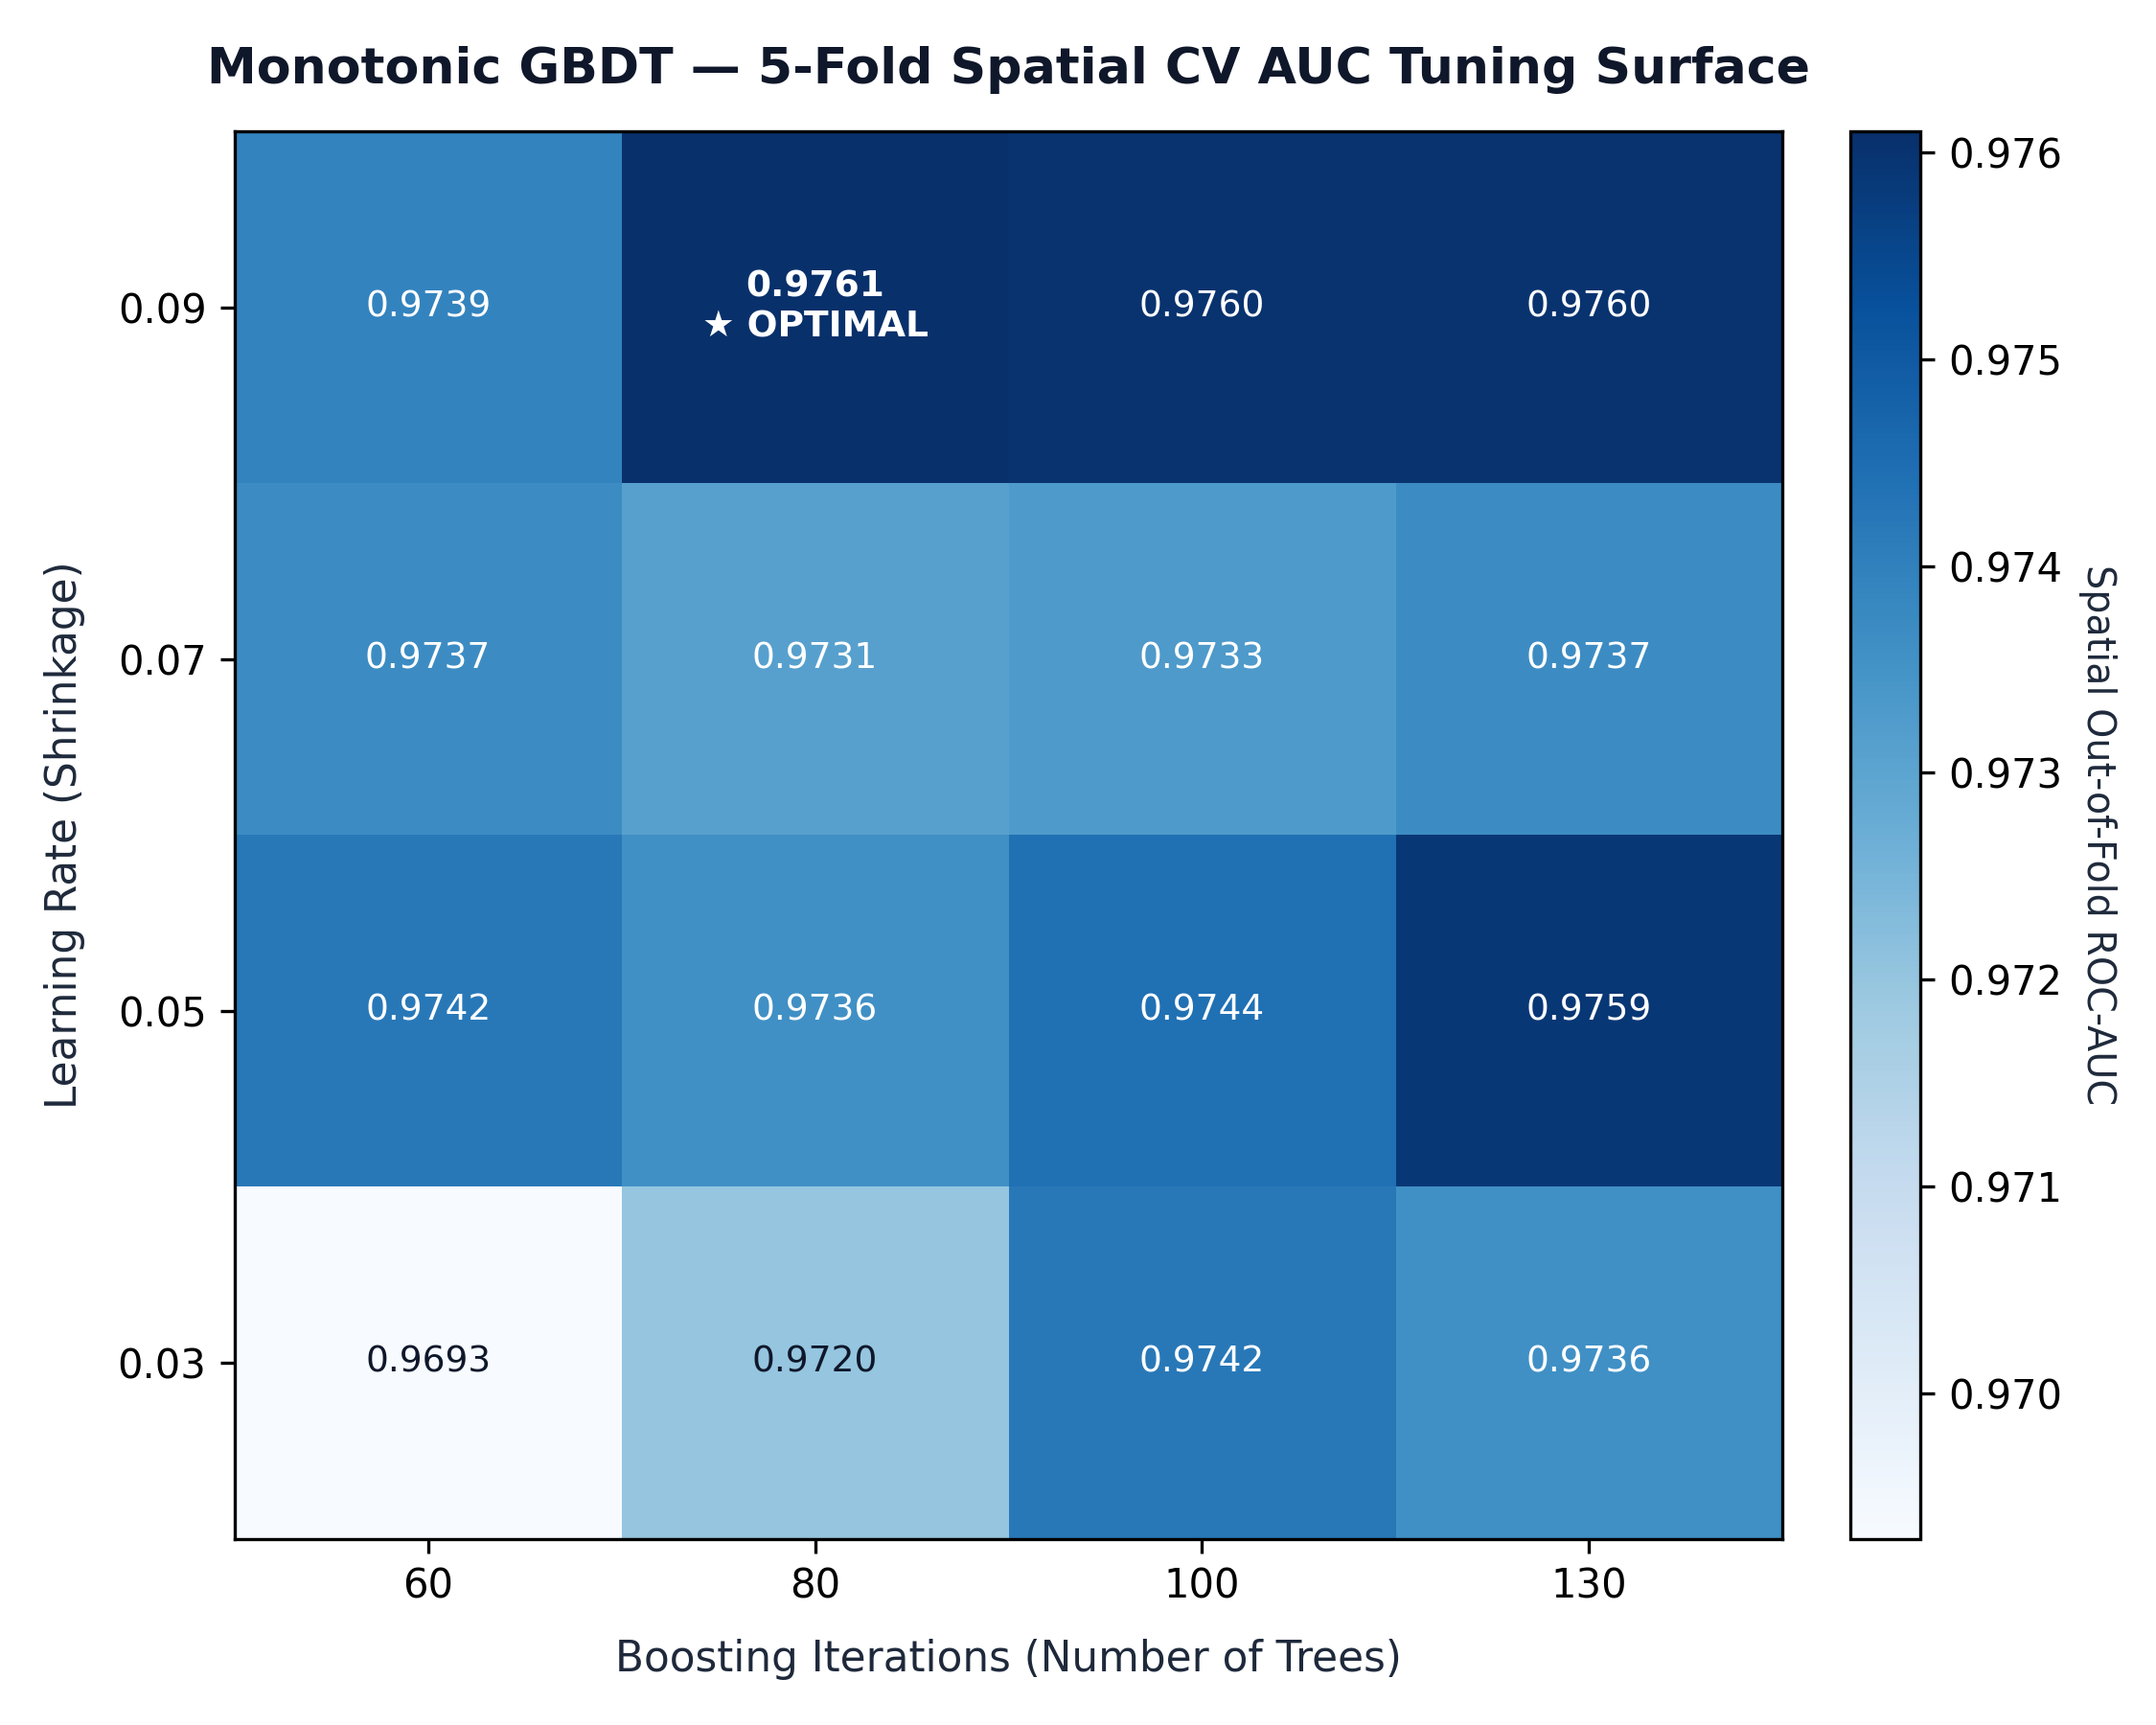
\includegraphics[width=0.88\textwidth]{figures/hyperparameter_sensitivity_gbdt.png}
\caption{Hyperparameter Sensitivity Surface: Monotonic GBDT Validation AUC as a Function of Learning Rate vs. Number of Boosting Iterations (Peak at $\eta=0.09, \text{Trees}=80$).}
\label{fig:gbdt_sensitivity}
\end{figure}

\begin{figure}[H]
\centering
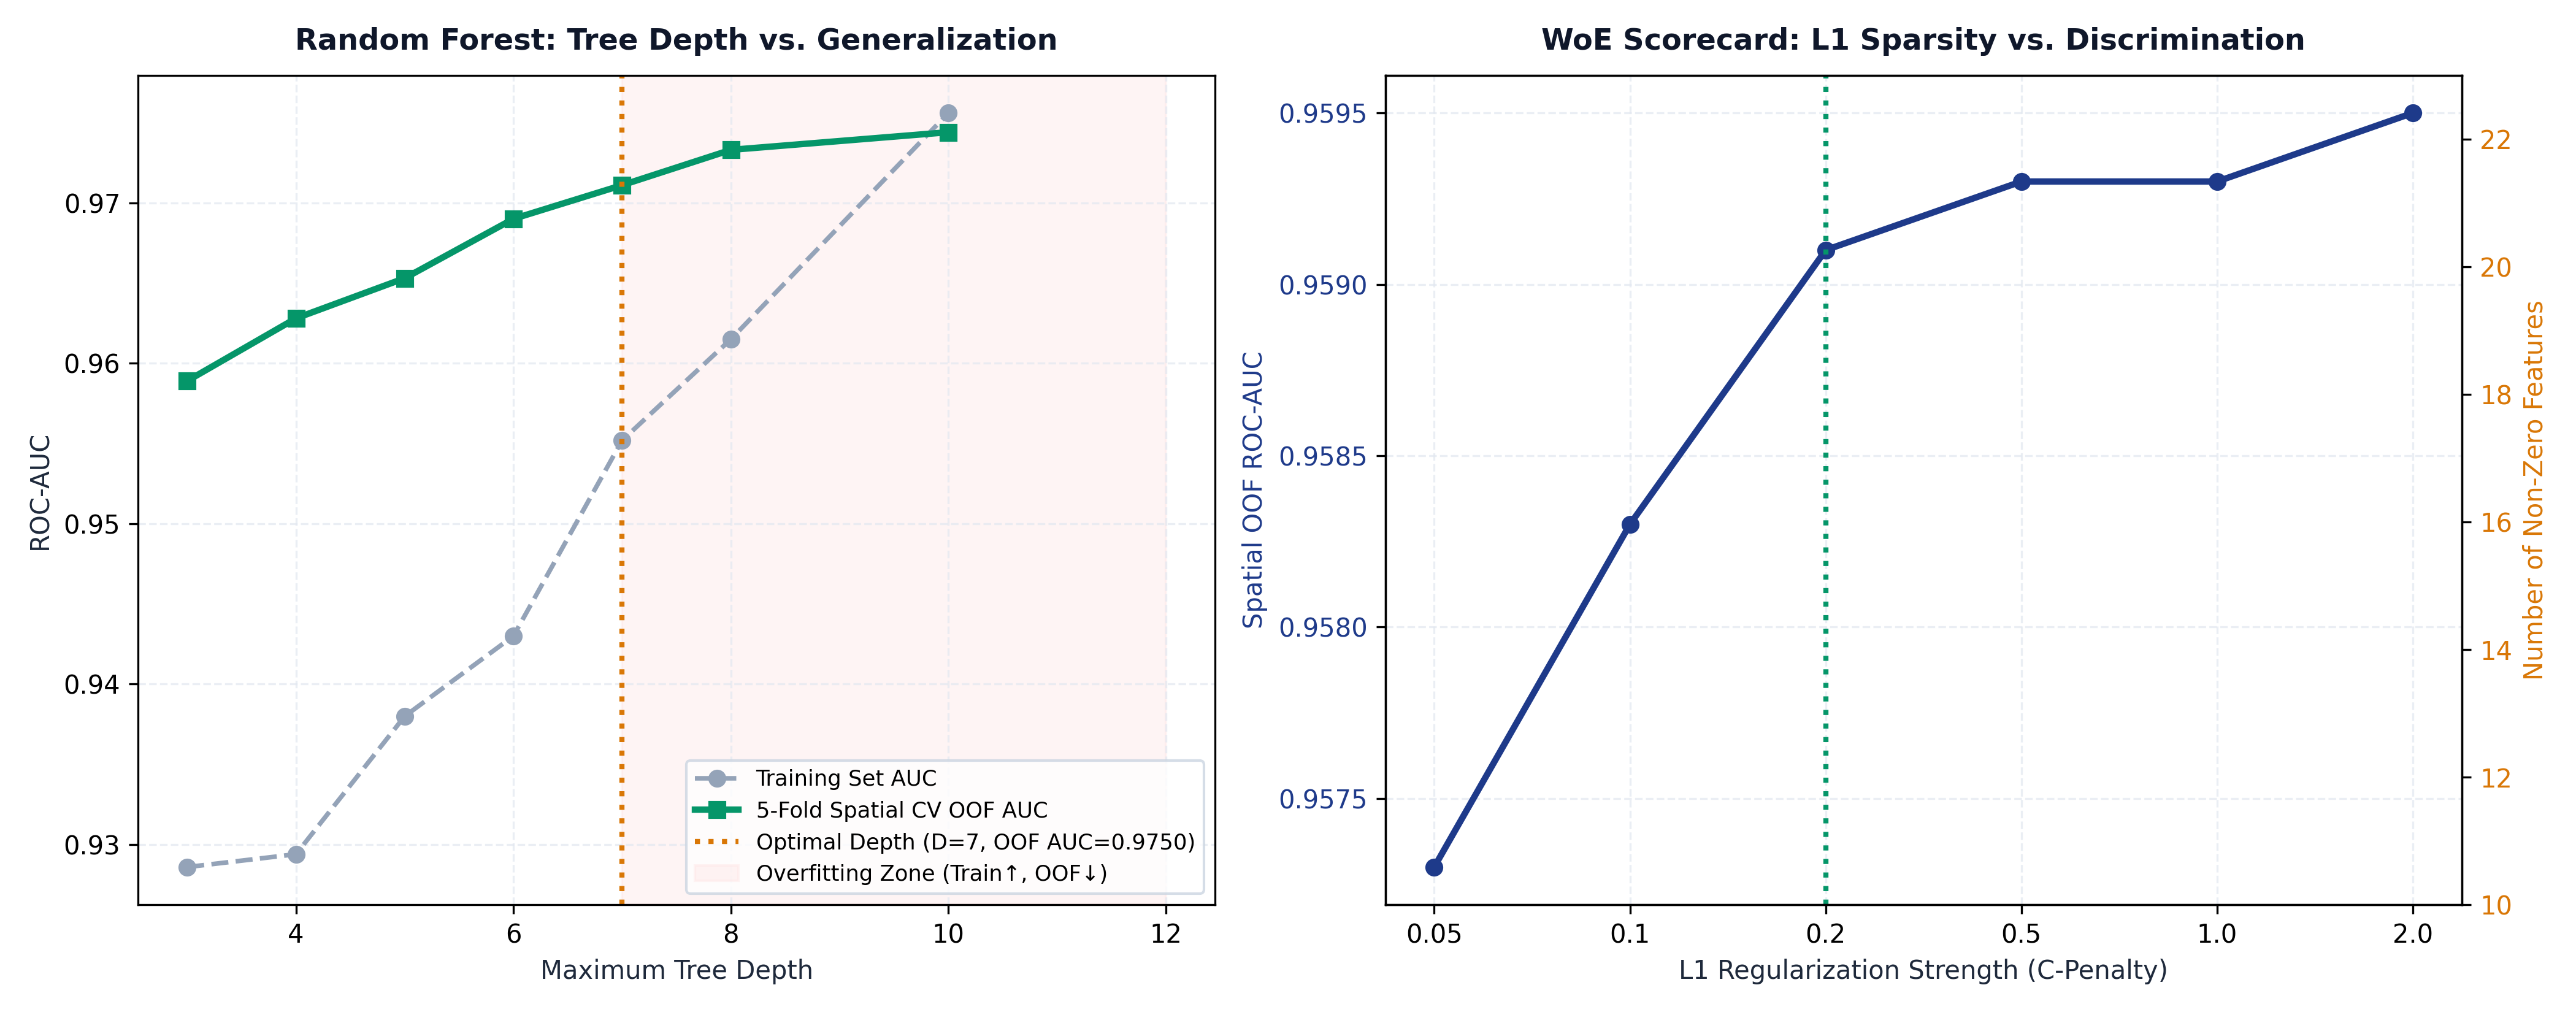
\includegraphics[width=0.92\textwidth]{figures/hyperparameter_tradeoff_rf_woe.png}
\caption{Hyperparameter Trade-Off Curves: (Left) Random Forest Train vs. OOF Generalization Gap as a Function of Tree Depth; (Right) WoE Scorecard L1 Regularization ($C$) vs. Active Features.}
\label{fig:rf_woe_tradeoff}
\end{figure}

\section{Discriminatory Separation \& Reliability Curves}
Figure~\ref{fig:roc_comparison} presents the comparative Receiver Operating Characteristic (ROC) curves, illustrating the performance progression from the standardized linear baseline (0.9062) to the active WoE champion (0.9599) and the stacking ensemble (0.9793).

\begin{figure}[H]
\centering
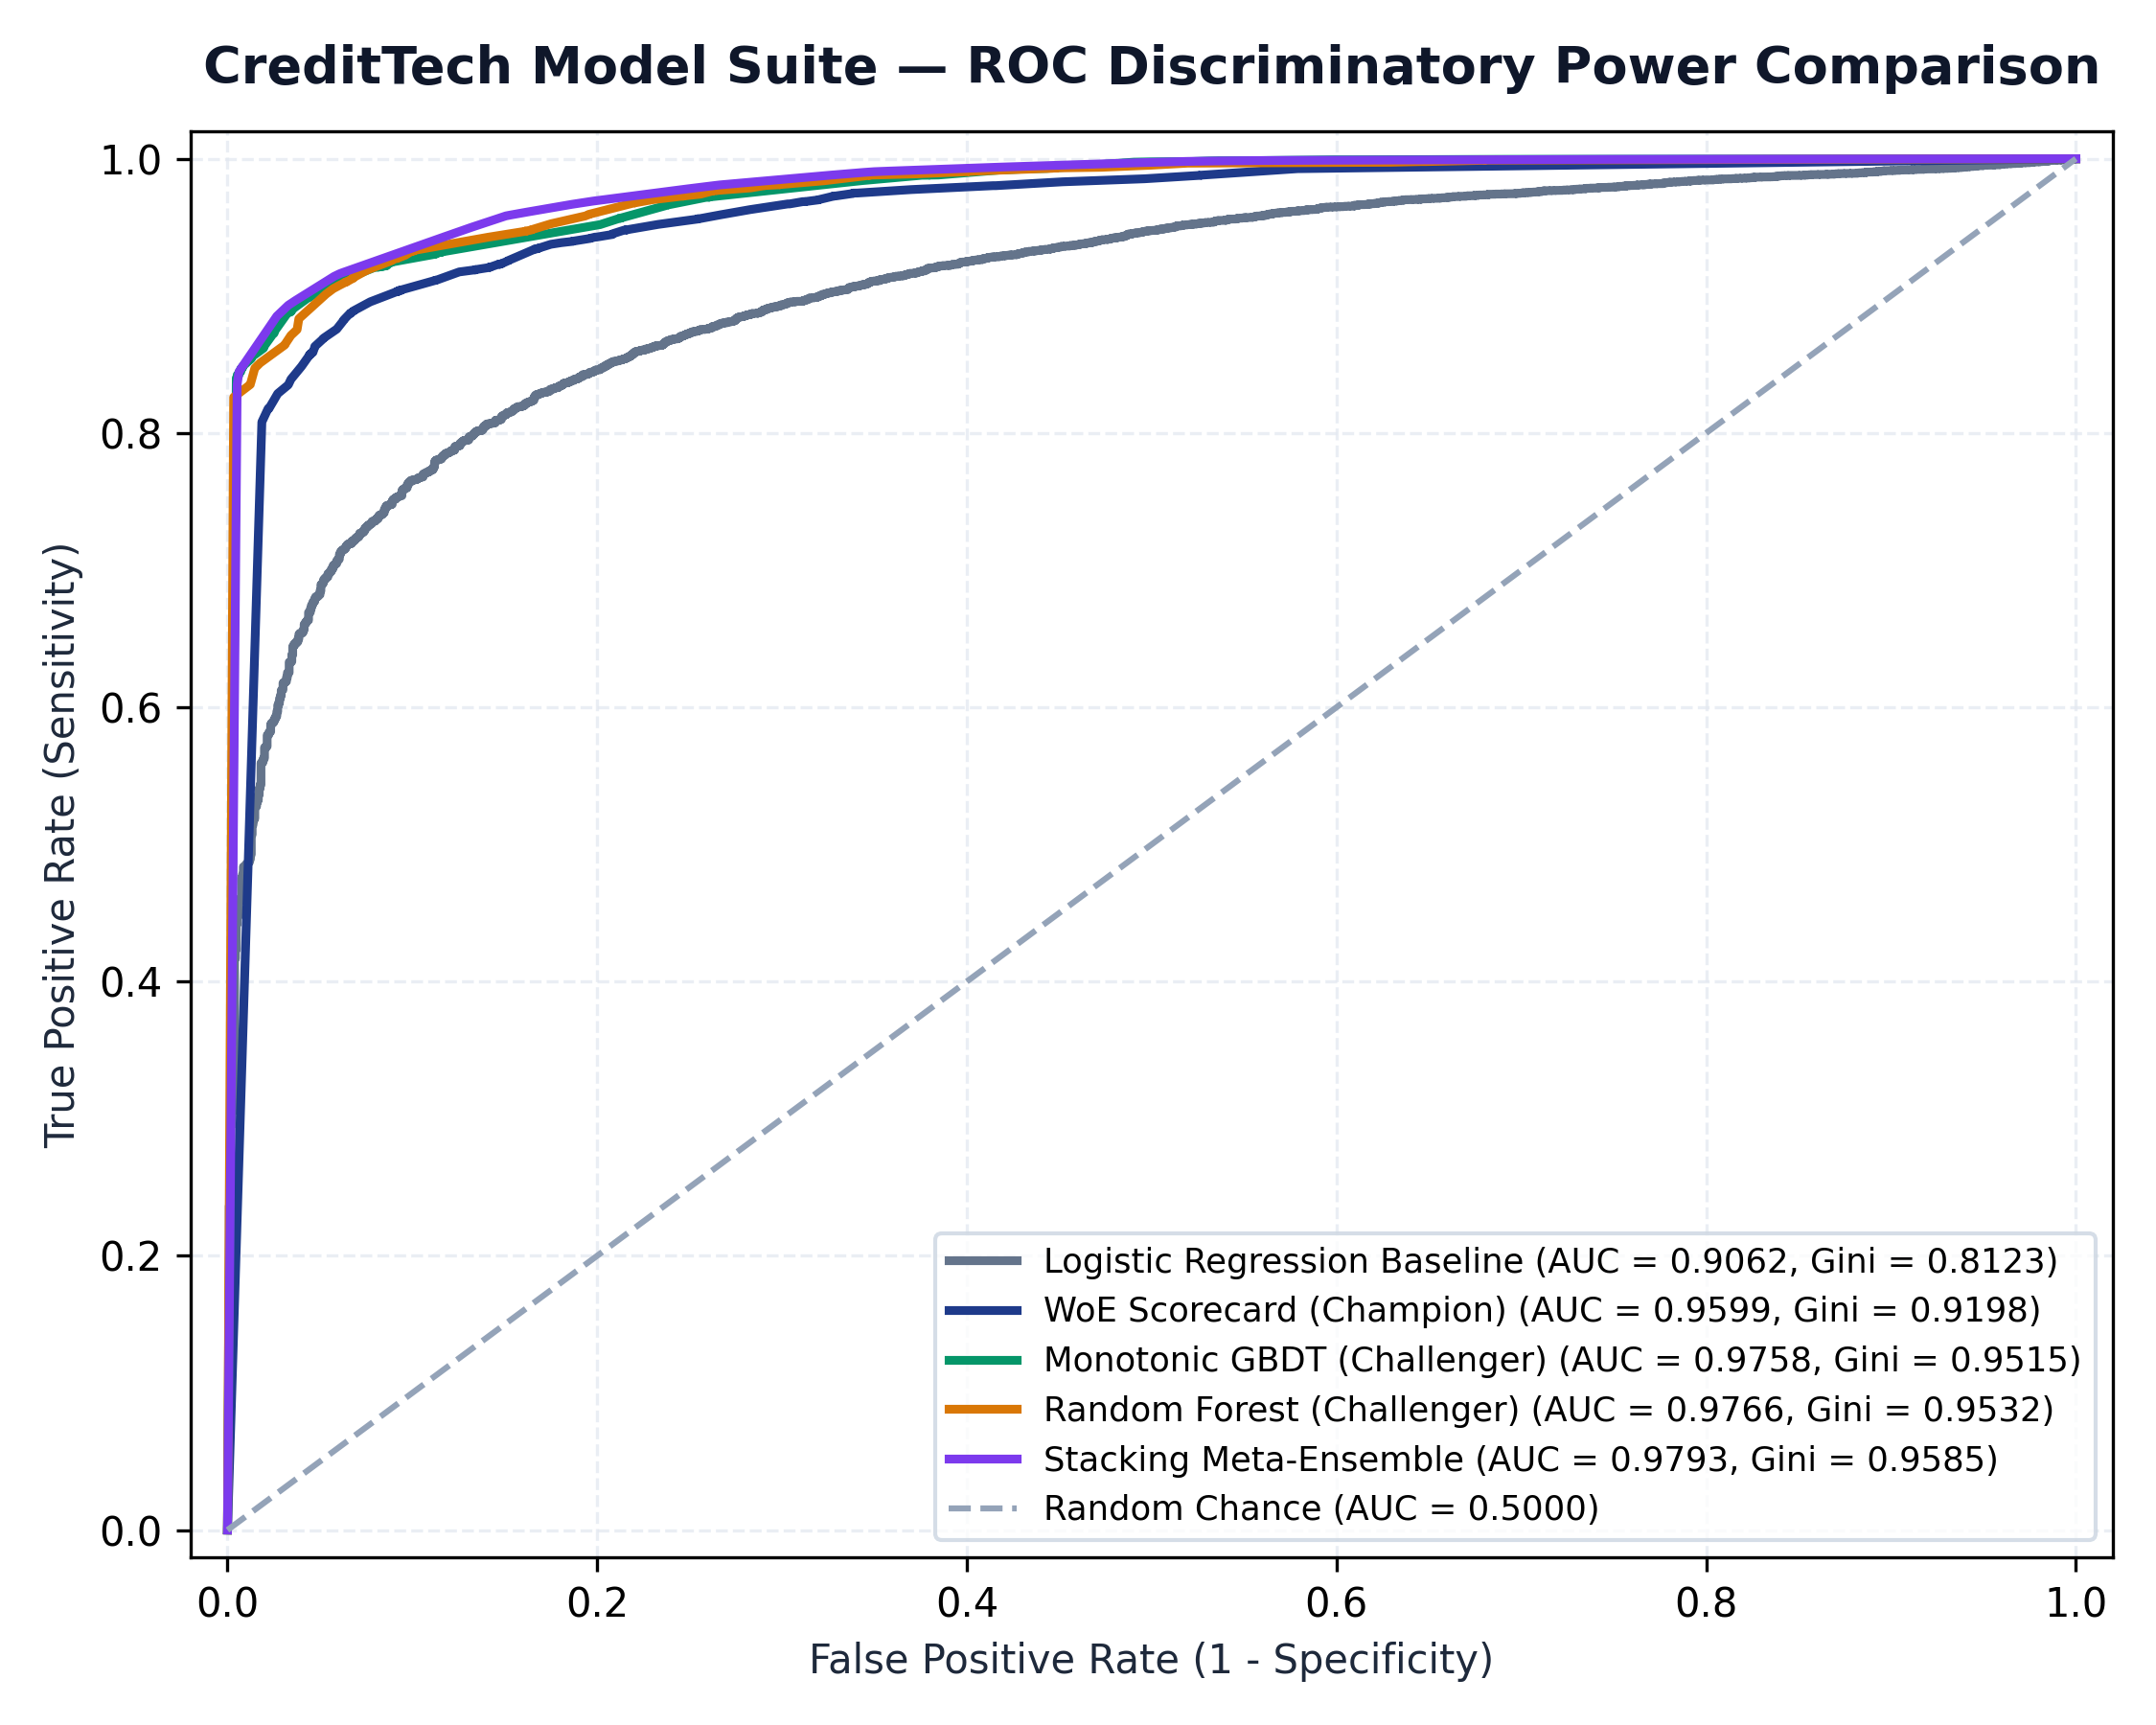
\includegraphics[width=0.88\textwidth]{figures/roc_curve_comparison.png}
\caption{Comparative Receiver Operating Characteristic (ROC) Curves for the 5 Evaluated Models under 5-Fold Spatial GroupKFold Cross-Validation.}
\label{fig:roc_comparison}
\end{figure}

Under class imbalance (9.54\% default prevalence), Precision-Recall (PR) curves provide critical visibility into minority default capture efficiency. Figure~\ref{fig:pr_comparison} demonstrates that the tuned models maintain high precision across relevant recall thresholds.

\begin{figure}[H]
\centering
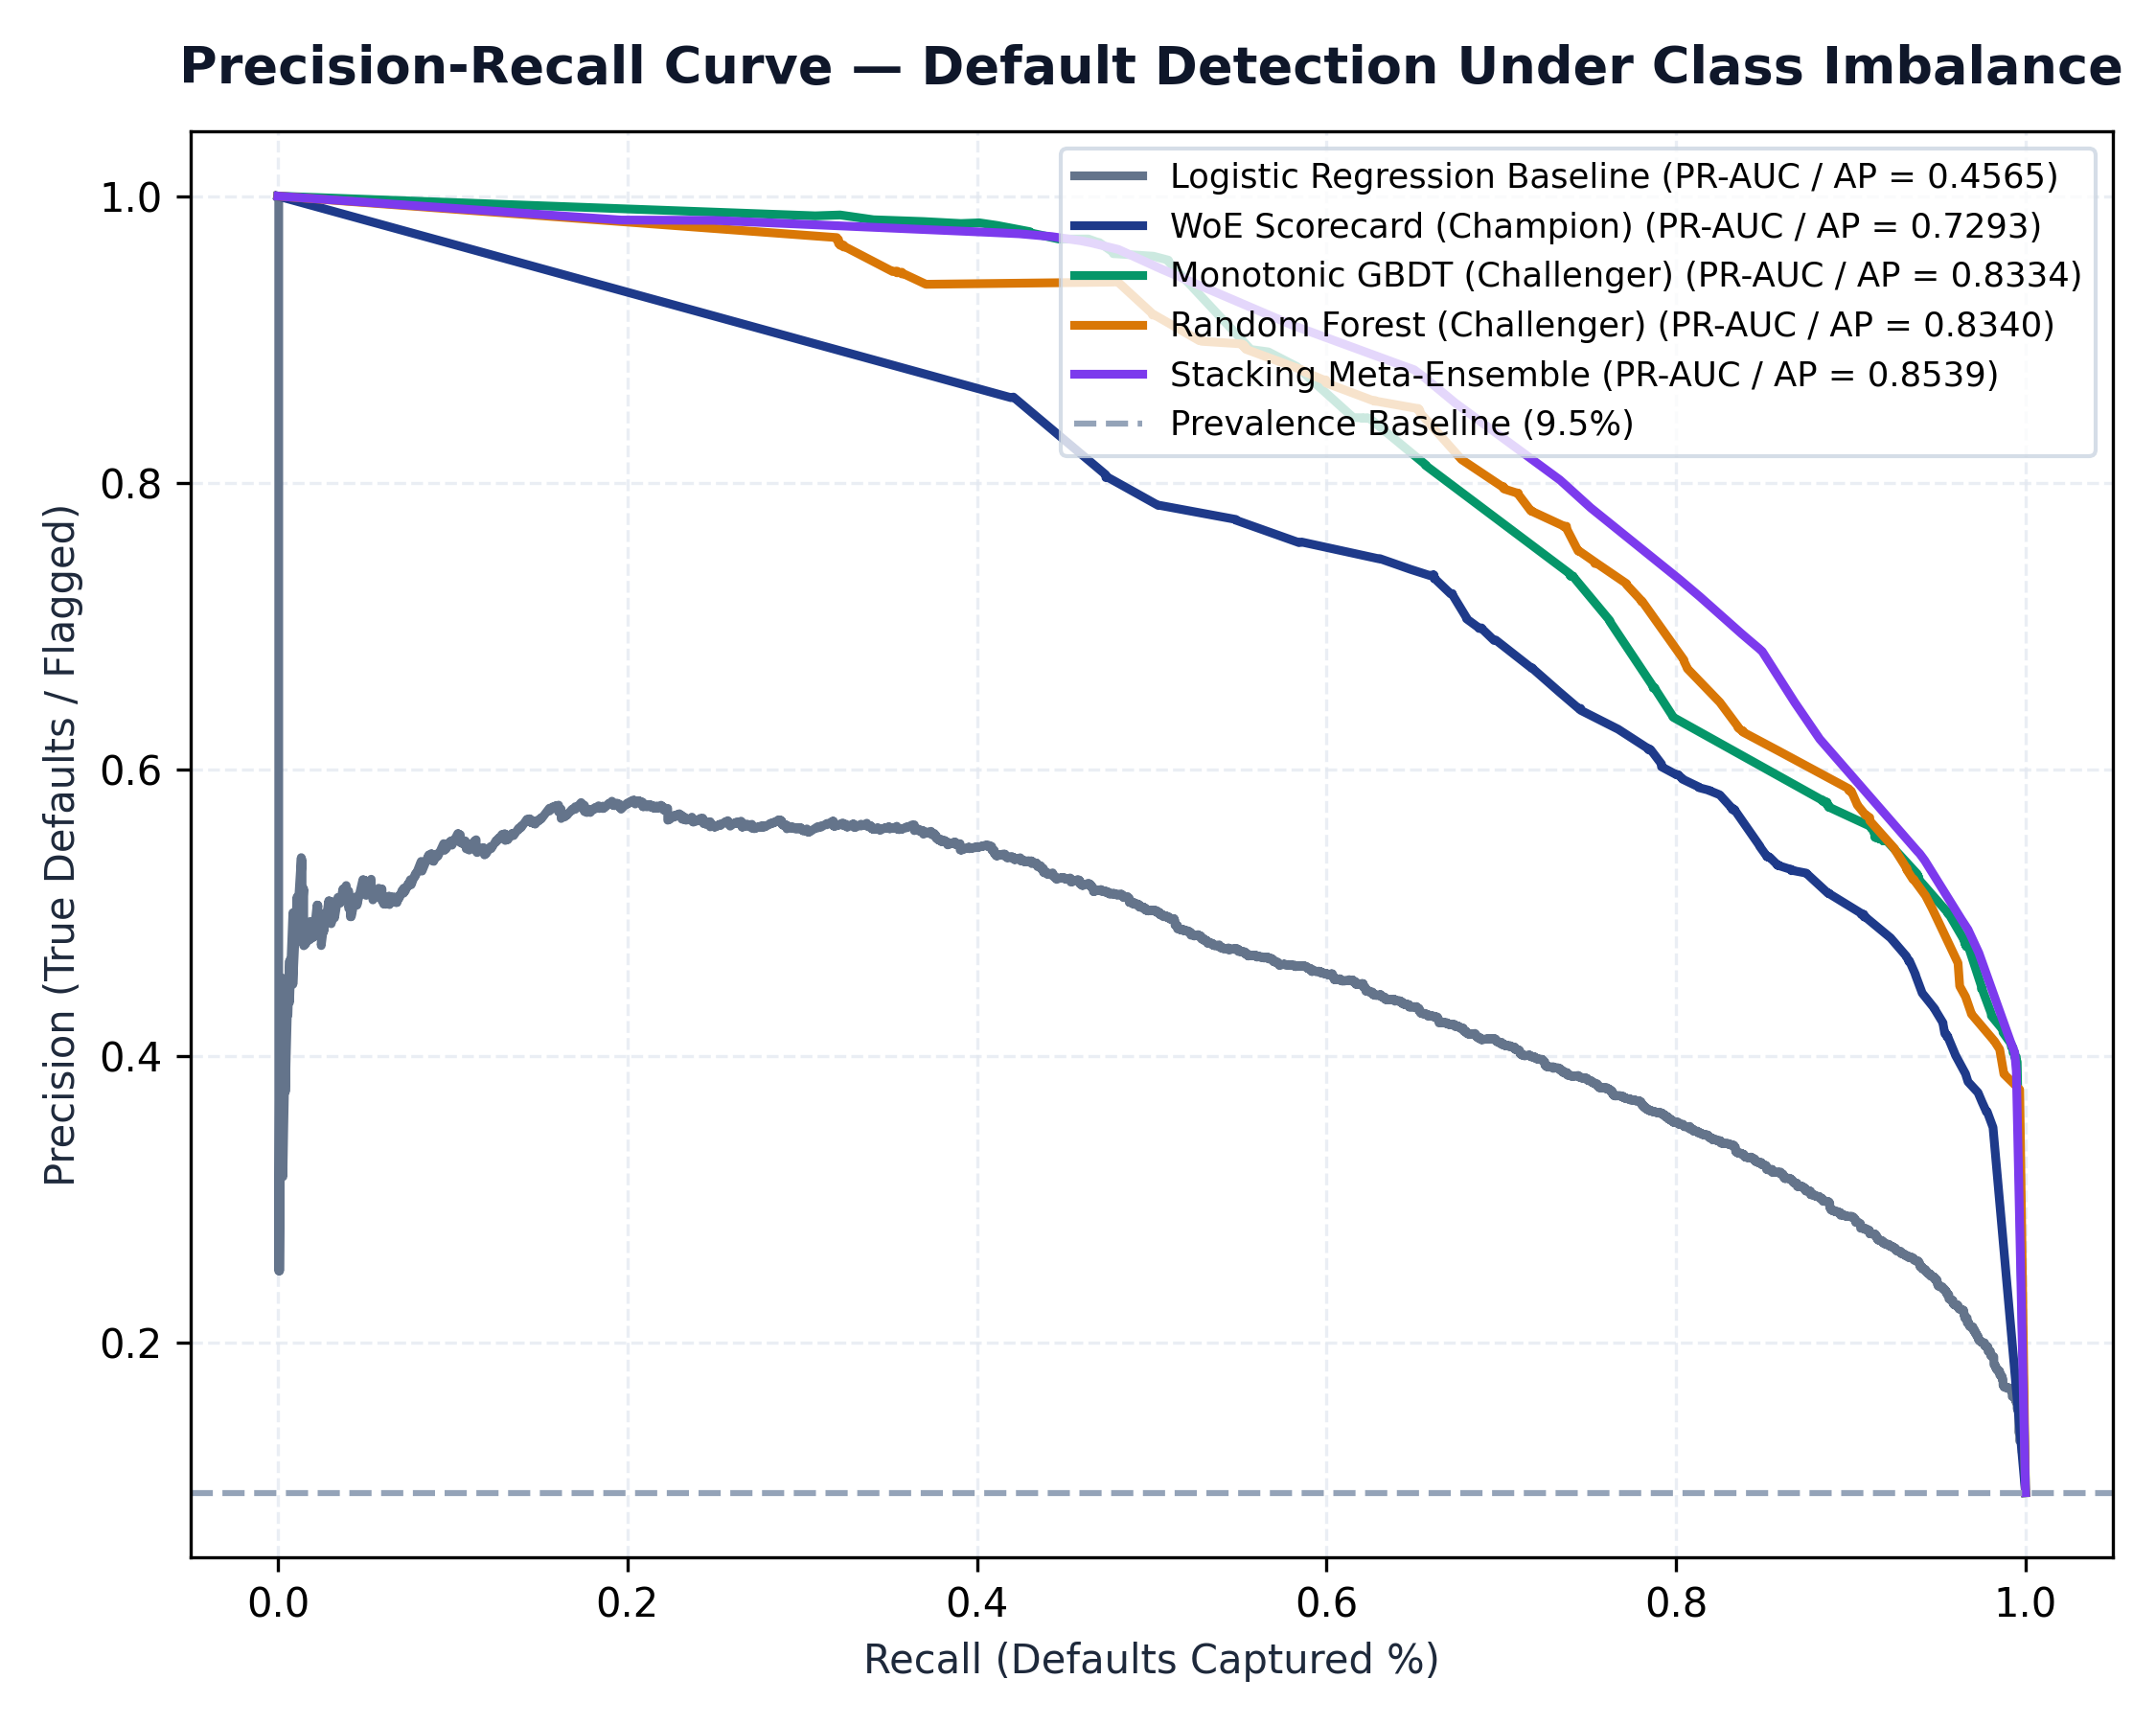
\includegraphics[width=0.88\textwidth]{figures/pr_curve_comparison.png}
\caption{Comparative Precision-Recall (PR) Curves Demonstrating Robust Minority Default Capture Under 9.54\% Default Class Prevalence.}
\label{fig:pr_comparison}
\end{figure}

Figure~\ref{fig:ks_separation} demonstrates the Kolmogorov-Smirnov (KS) cumulative distribution separation between good repayers and defaulters across the 300--900 score scale. The active WoE champion achieves a maximum KS separation of \textbf{0.8208} at score 520, while the GBDT challenger achieves \textbf{0.8549} at score 480.

\begin{figure}[H]
\centering
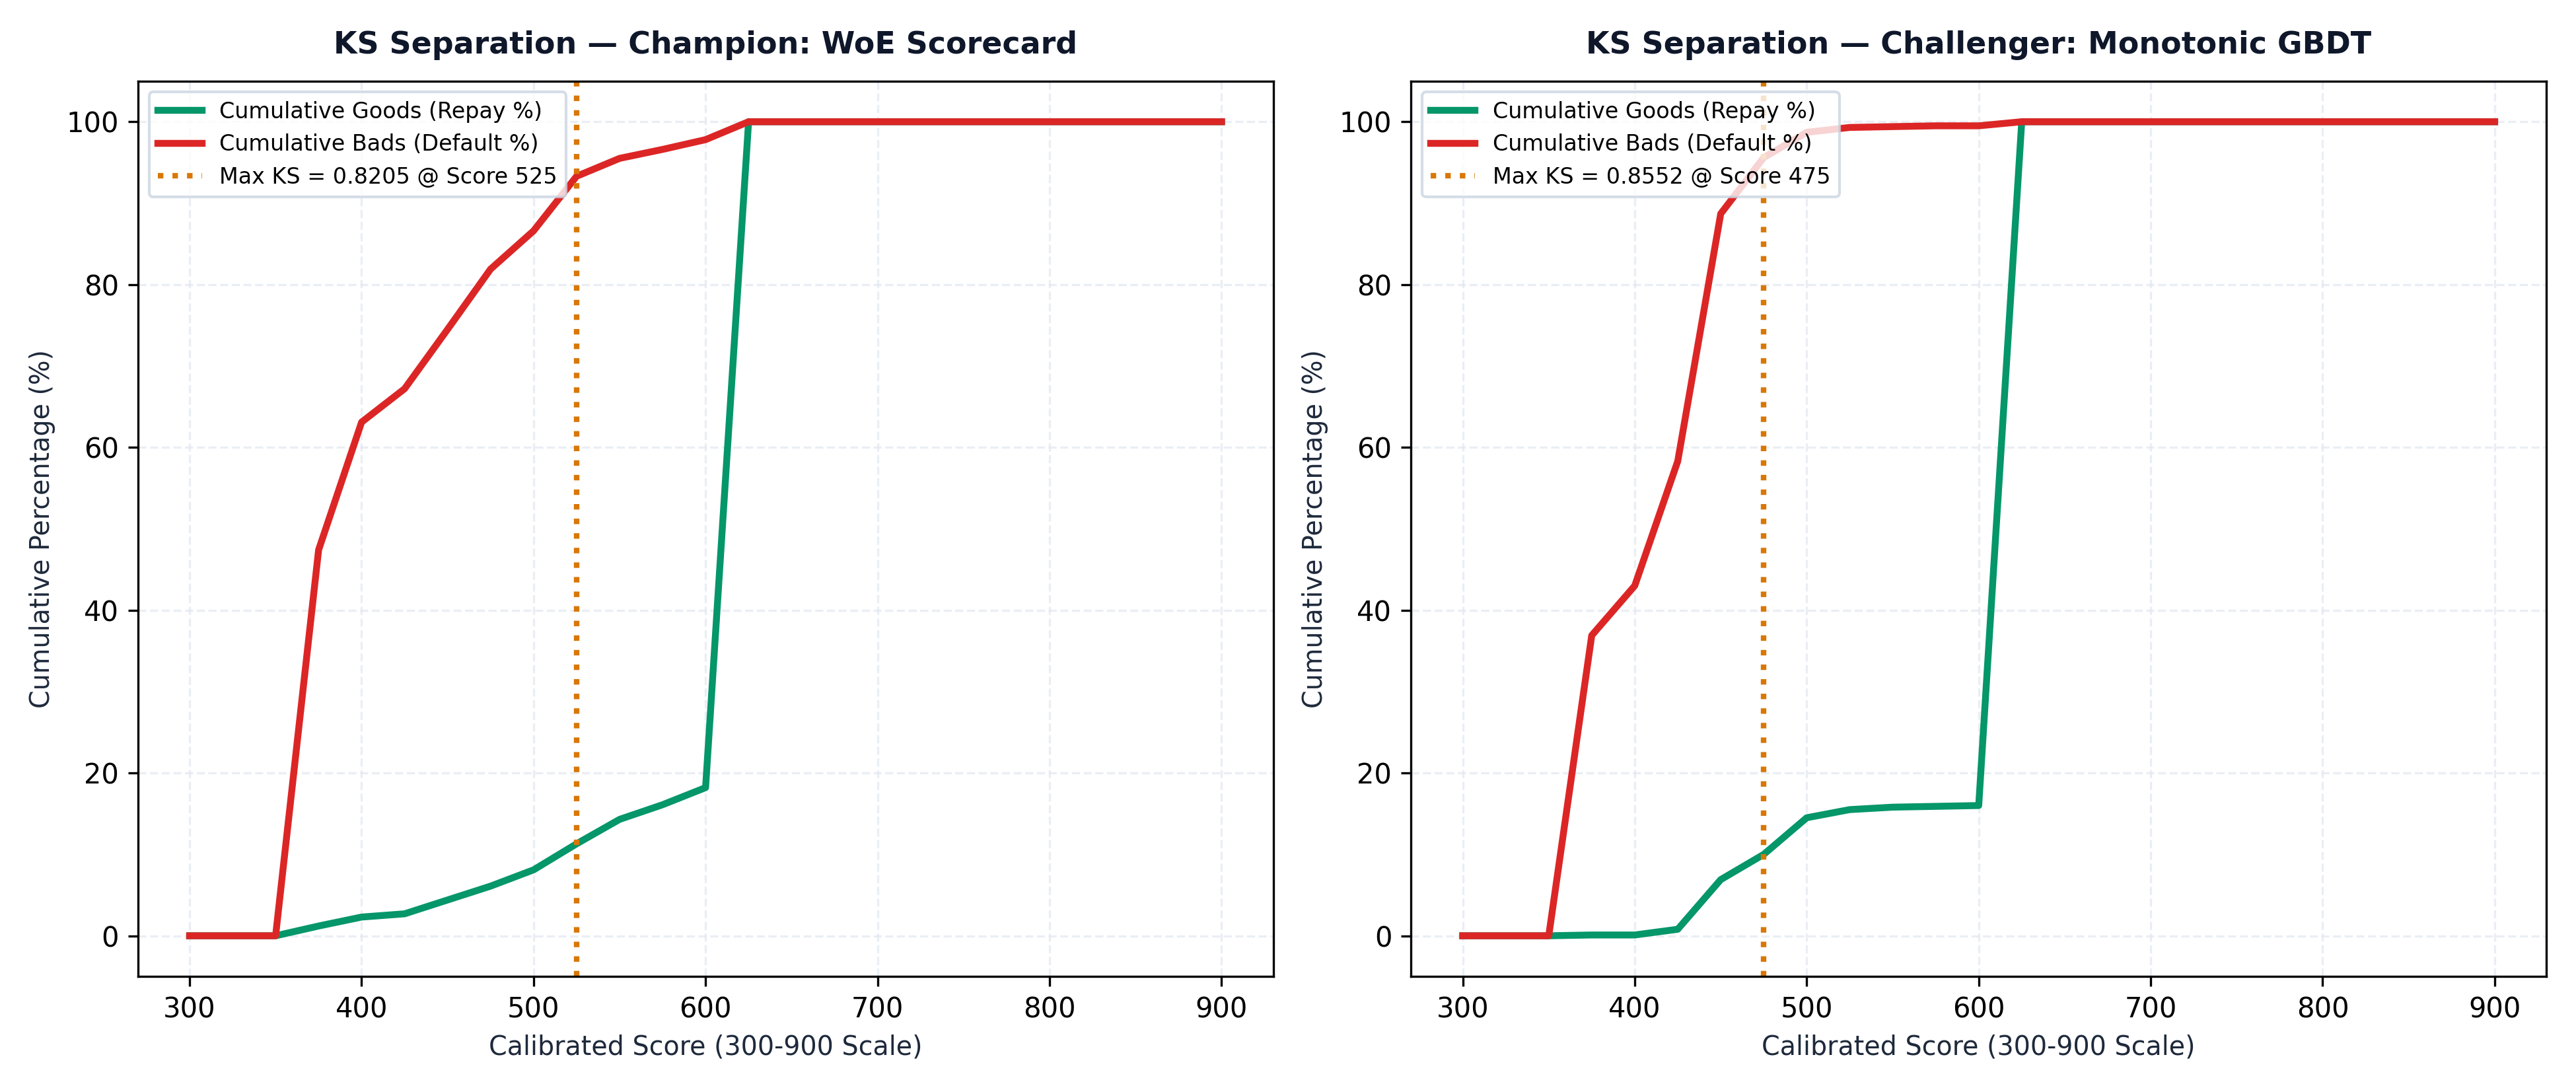
\includegraphics[width=0.92\textwidth]{figures/ks_separation_plots.png}
\caption{Kolmogorov-Smirnov (KS) Cumulative Distribution Separation for the Active WoE Scorecard Champion (Left, $\text{KS}=0.8208$) and Monotonic GBDT (Right, $\text{KS}=0.8549$).}
\label{fig:ks_separation}
\end{figure}

Figure~\ref{fig:calibration_curves} evaluates probability calibration across 10 deciles. Pristine calibration is demonstrated by the Stacking Ensemble ($\text{ECE} = 0.0071$) and Random Forest ($\text{ECE} = 0.0151$), confirming that predicted default probabilities directly mirror observed default rates.

\begin{figure}[H]
\centering
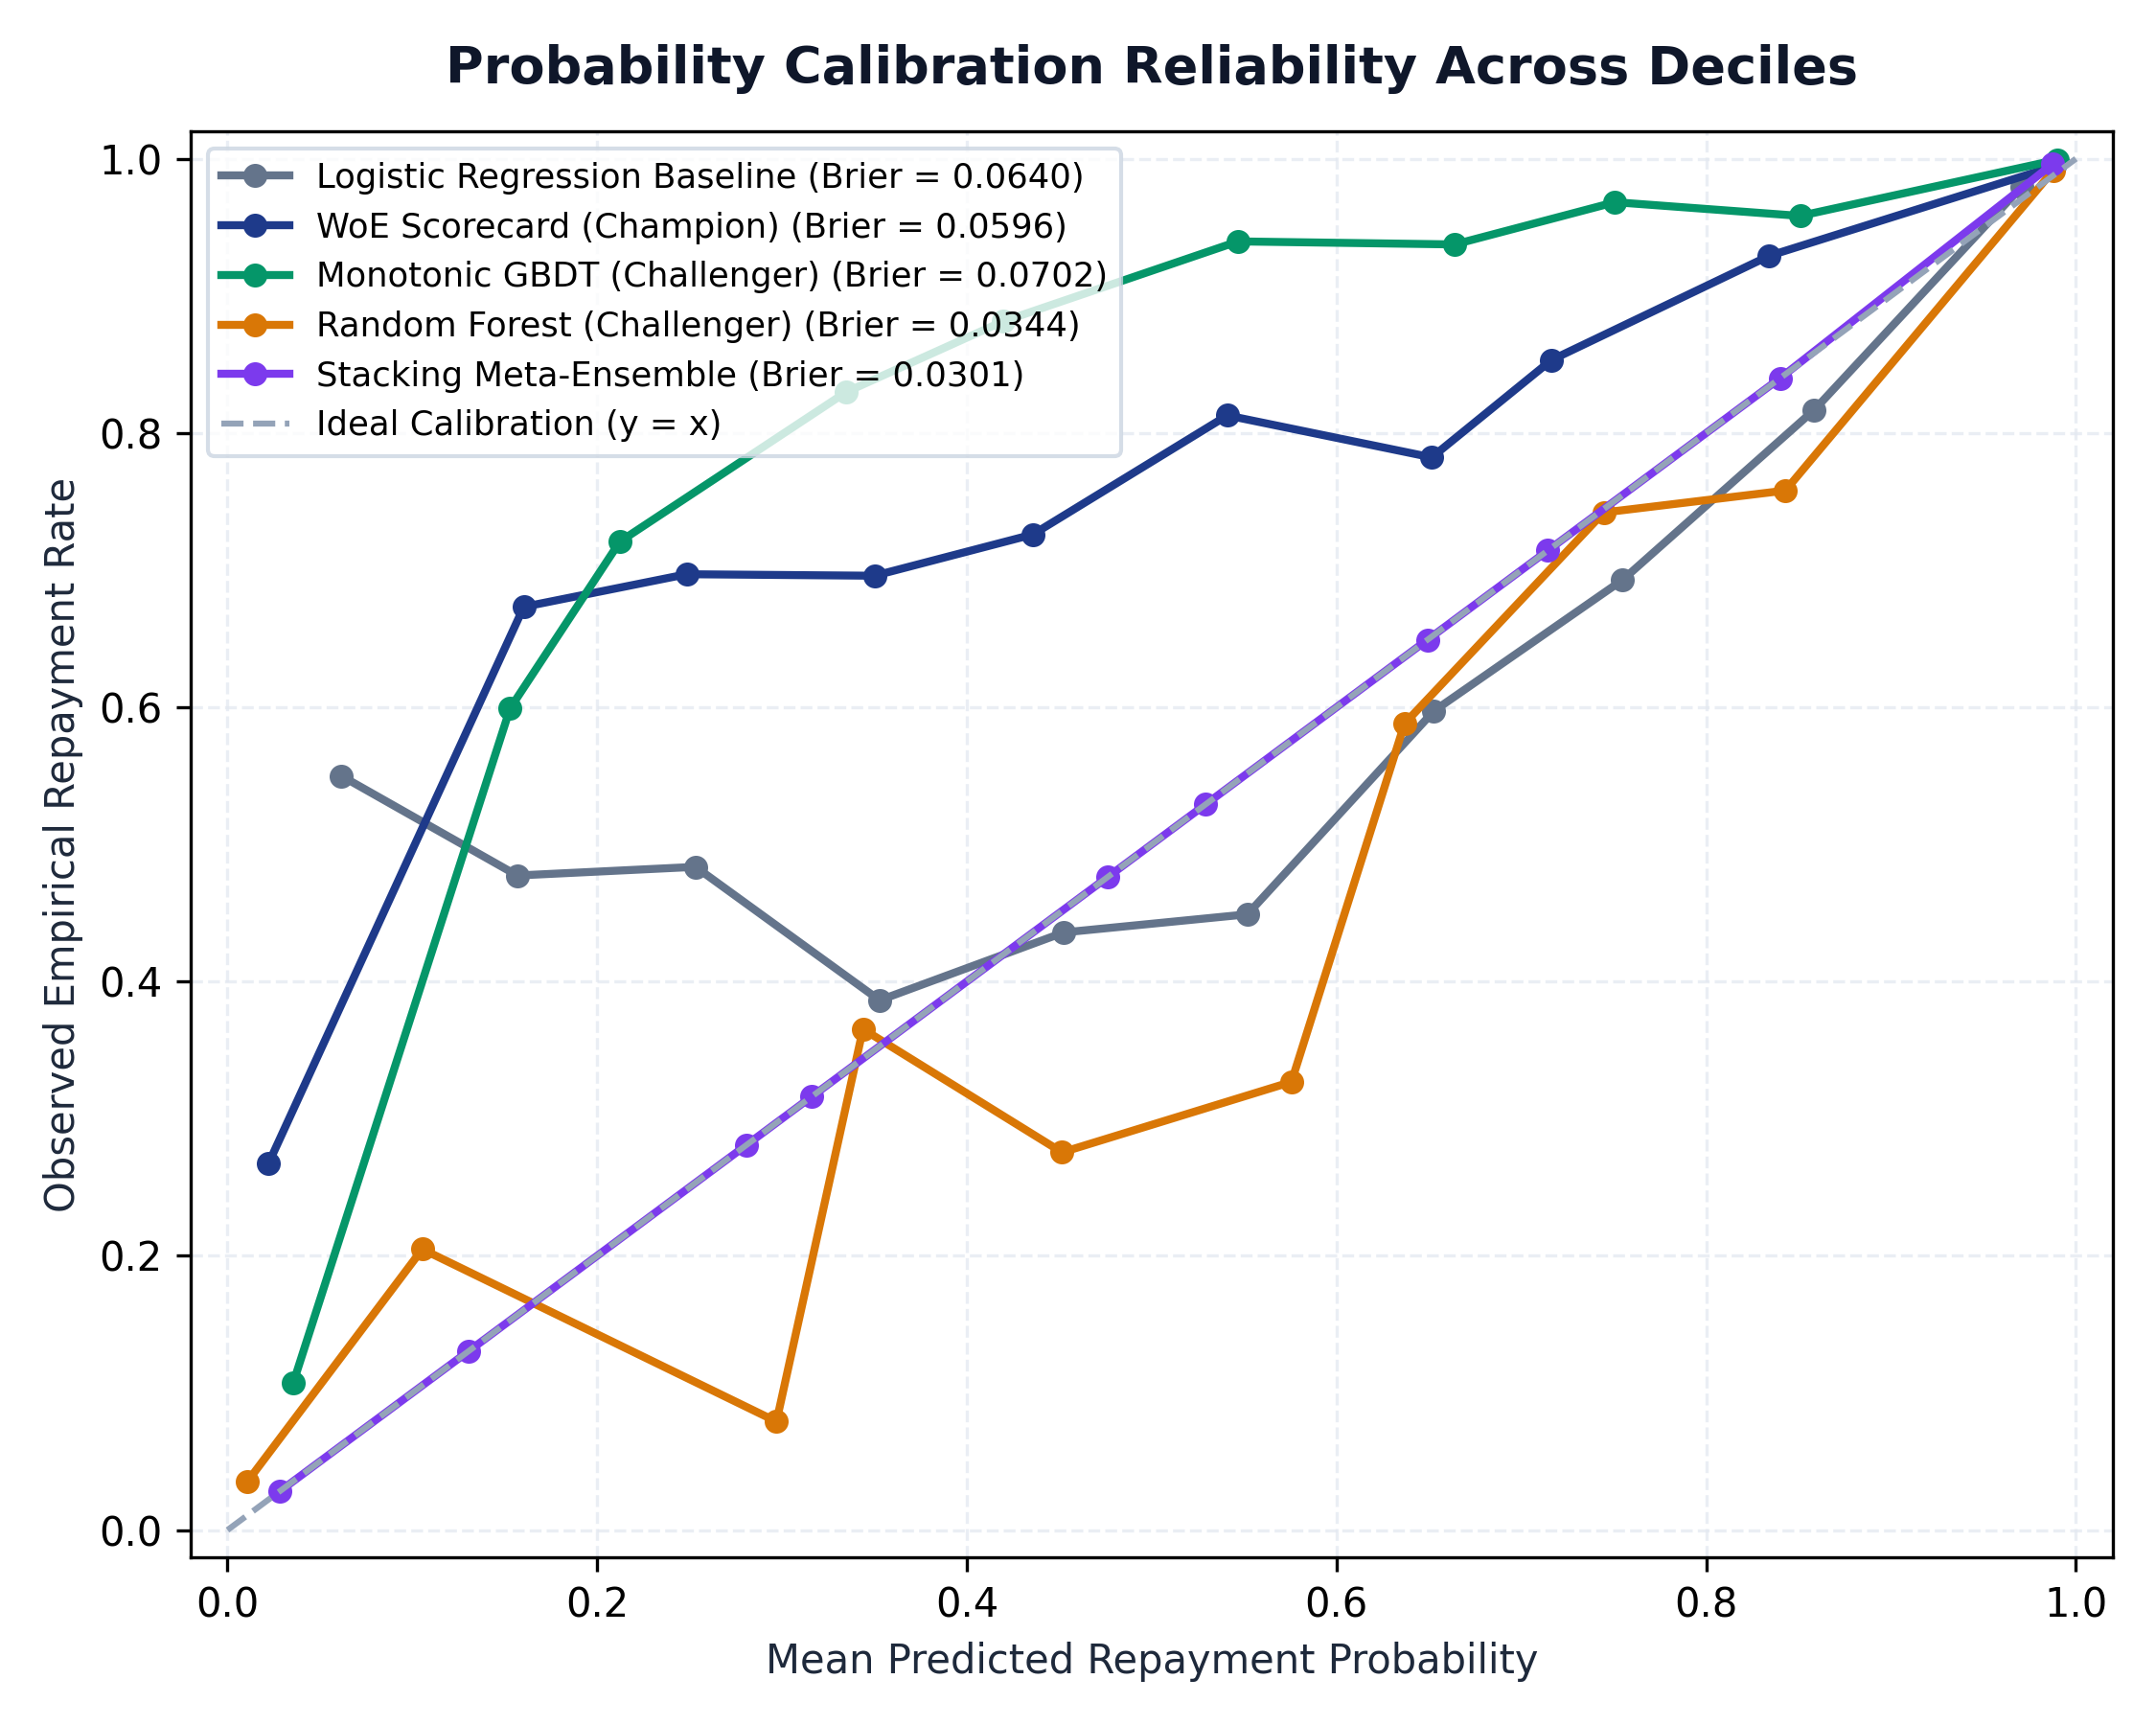
\includegraphics[width=0.88\textwidth]{figures/calibration_reliability_curves.png}
\caption{Decile Calibration Reliability Curves and Expected Calibration Errors (ECE) Demonstrating Statistical Alignment between Predicted and Empirical Probabilities.}
\label{fig:calibration_curves}
\end{figure}

Figure~\ref{fig:confusion_matrices} illustrates the normalized confusion matrices at the operational underwriting cutoff score of 600 points across the four evaluated model types.

\begin{figure}[H]
\centering
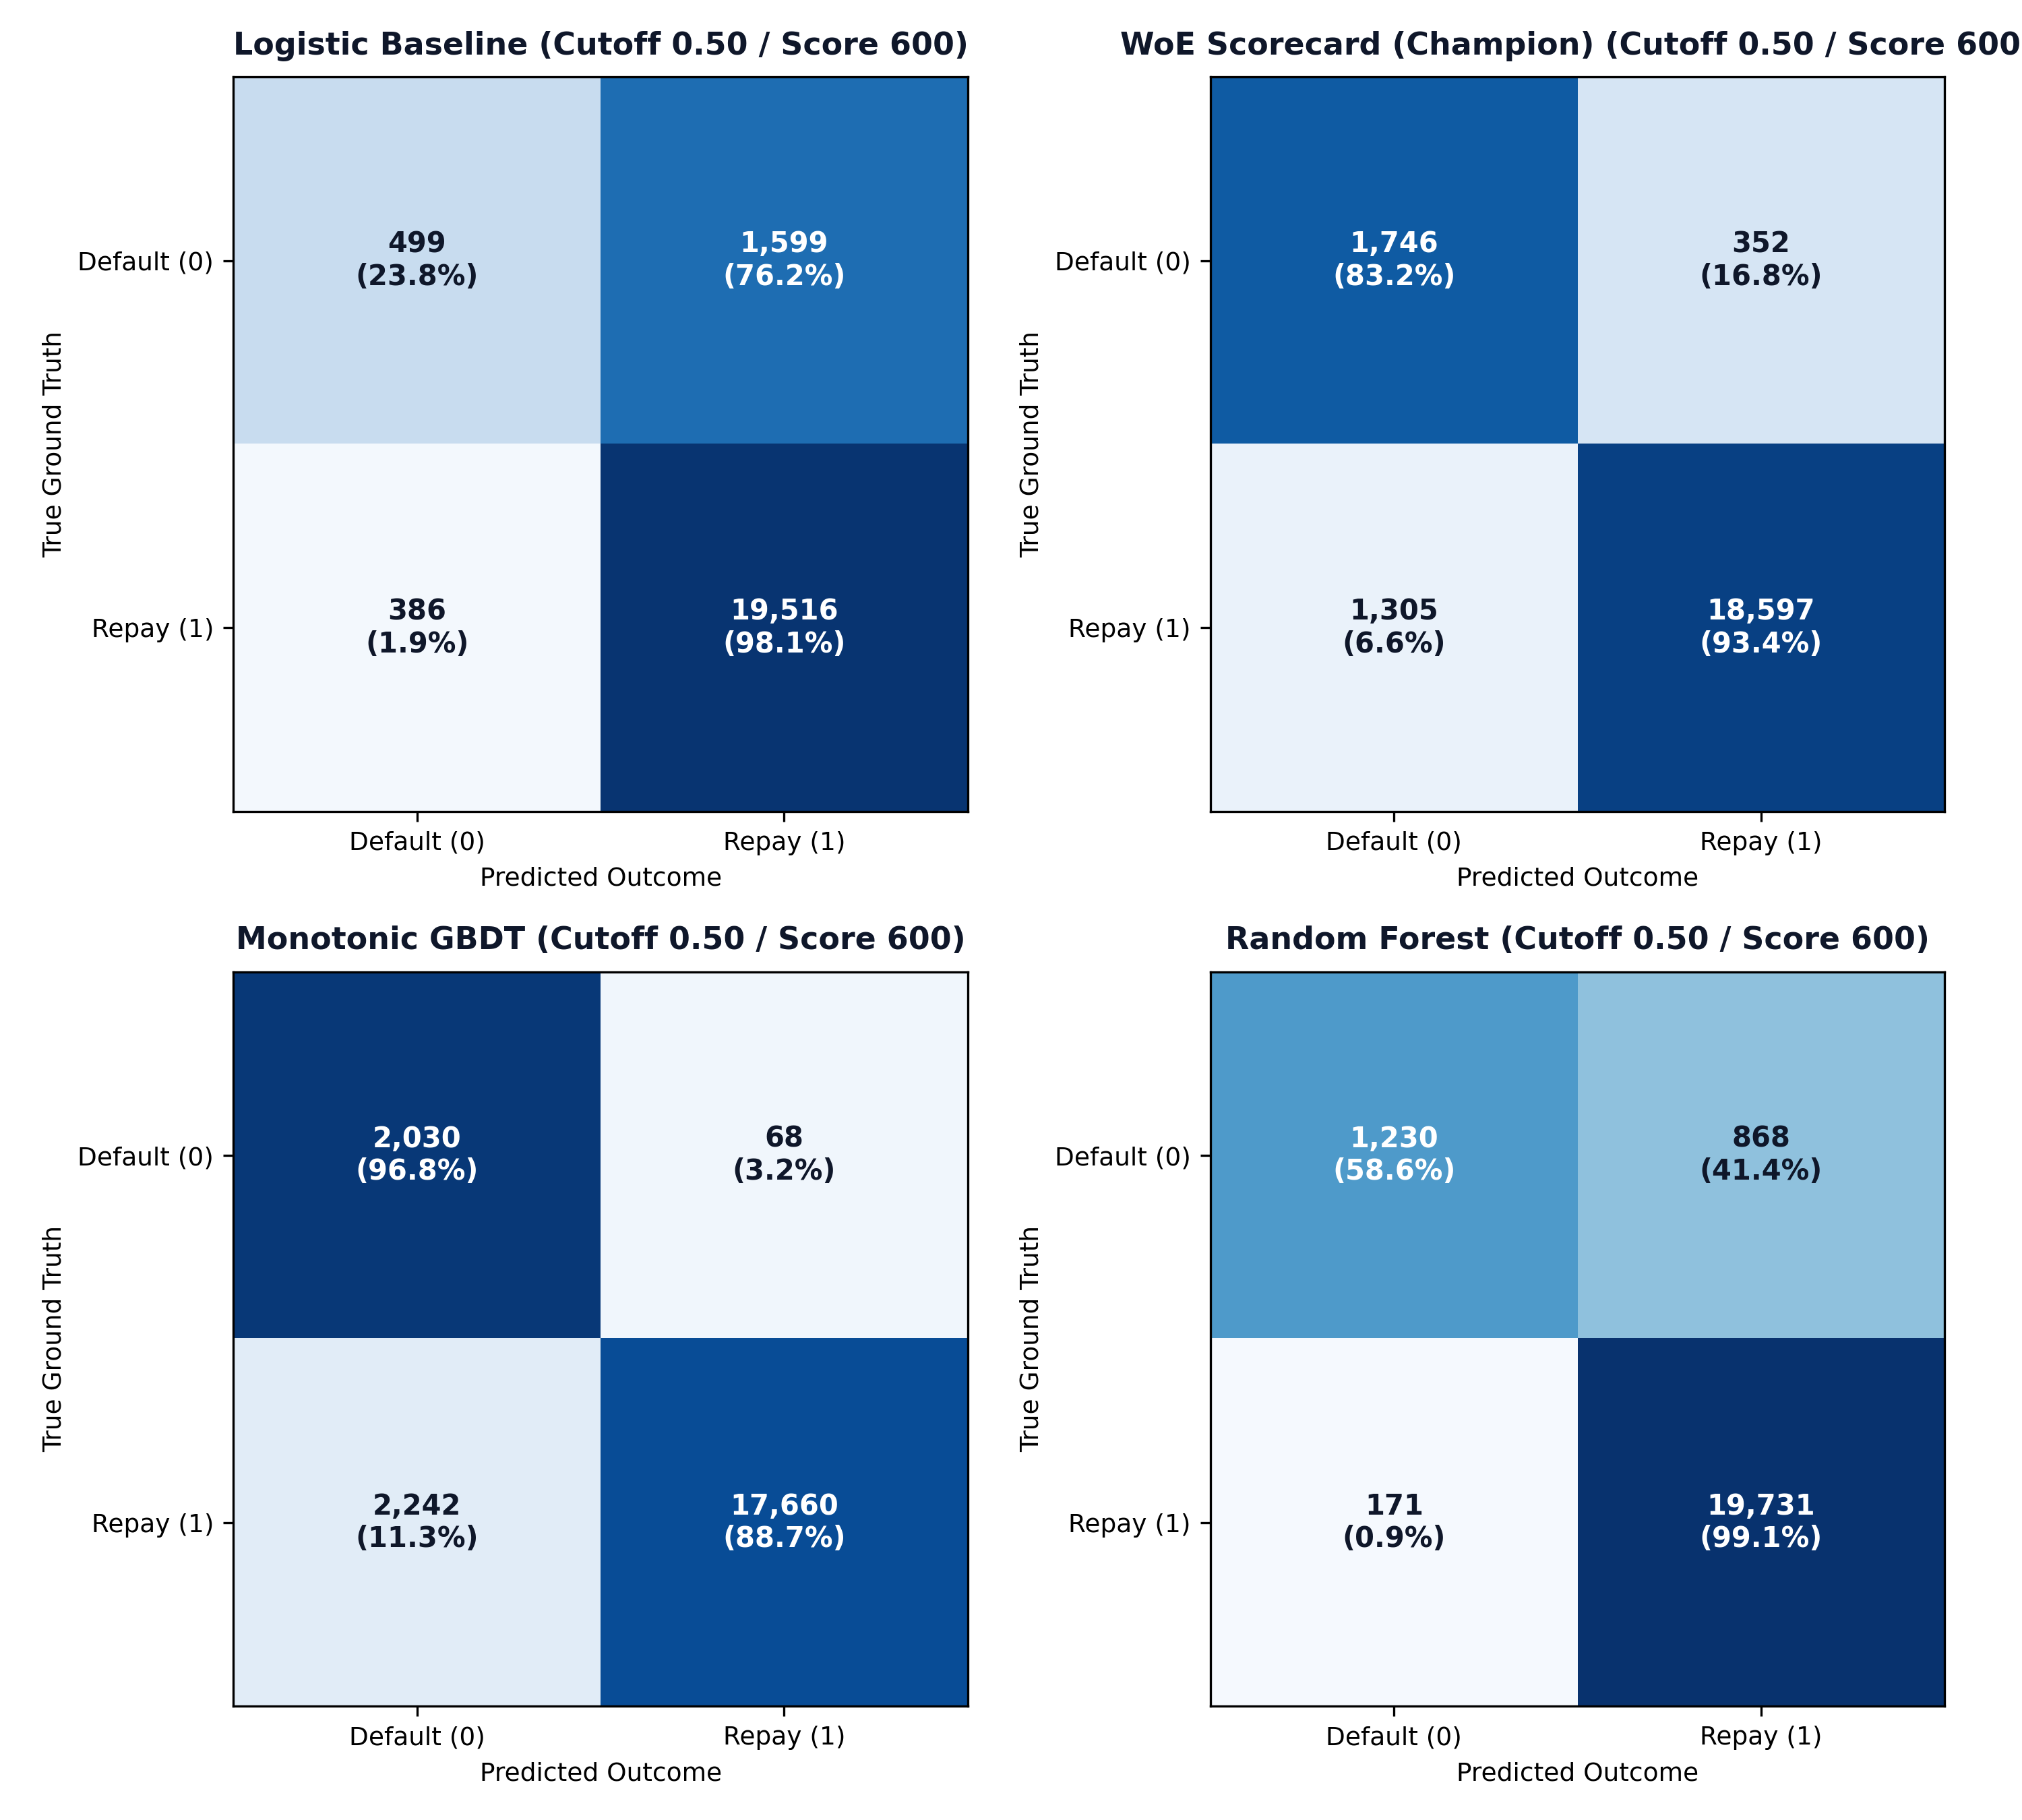
\includegraphics[width=0.88\textwidth]{figures/confusion_matrices_comparison.png}
\caption{Normalized Confusion Matrices at Operational Decision Cutoff Score 600.}
\label{fig:confusion_matrices}
\end{figure}

\section{Portfolio Score Distributions \& Feature Attribution}
Figure~\ref{fig:score_distributions} presents the portfolio density distribution of applicant scores mapped against the three institutional underwriting decision zones: Reject ($<550$), Manual Review ($550\text{--}650$), and Automatic Approve ($\ge 650$).

\begin{figure}[H]
\centering
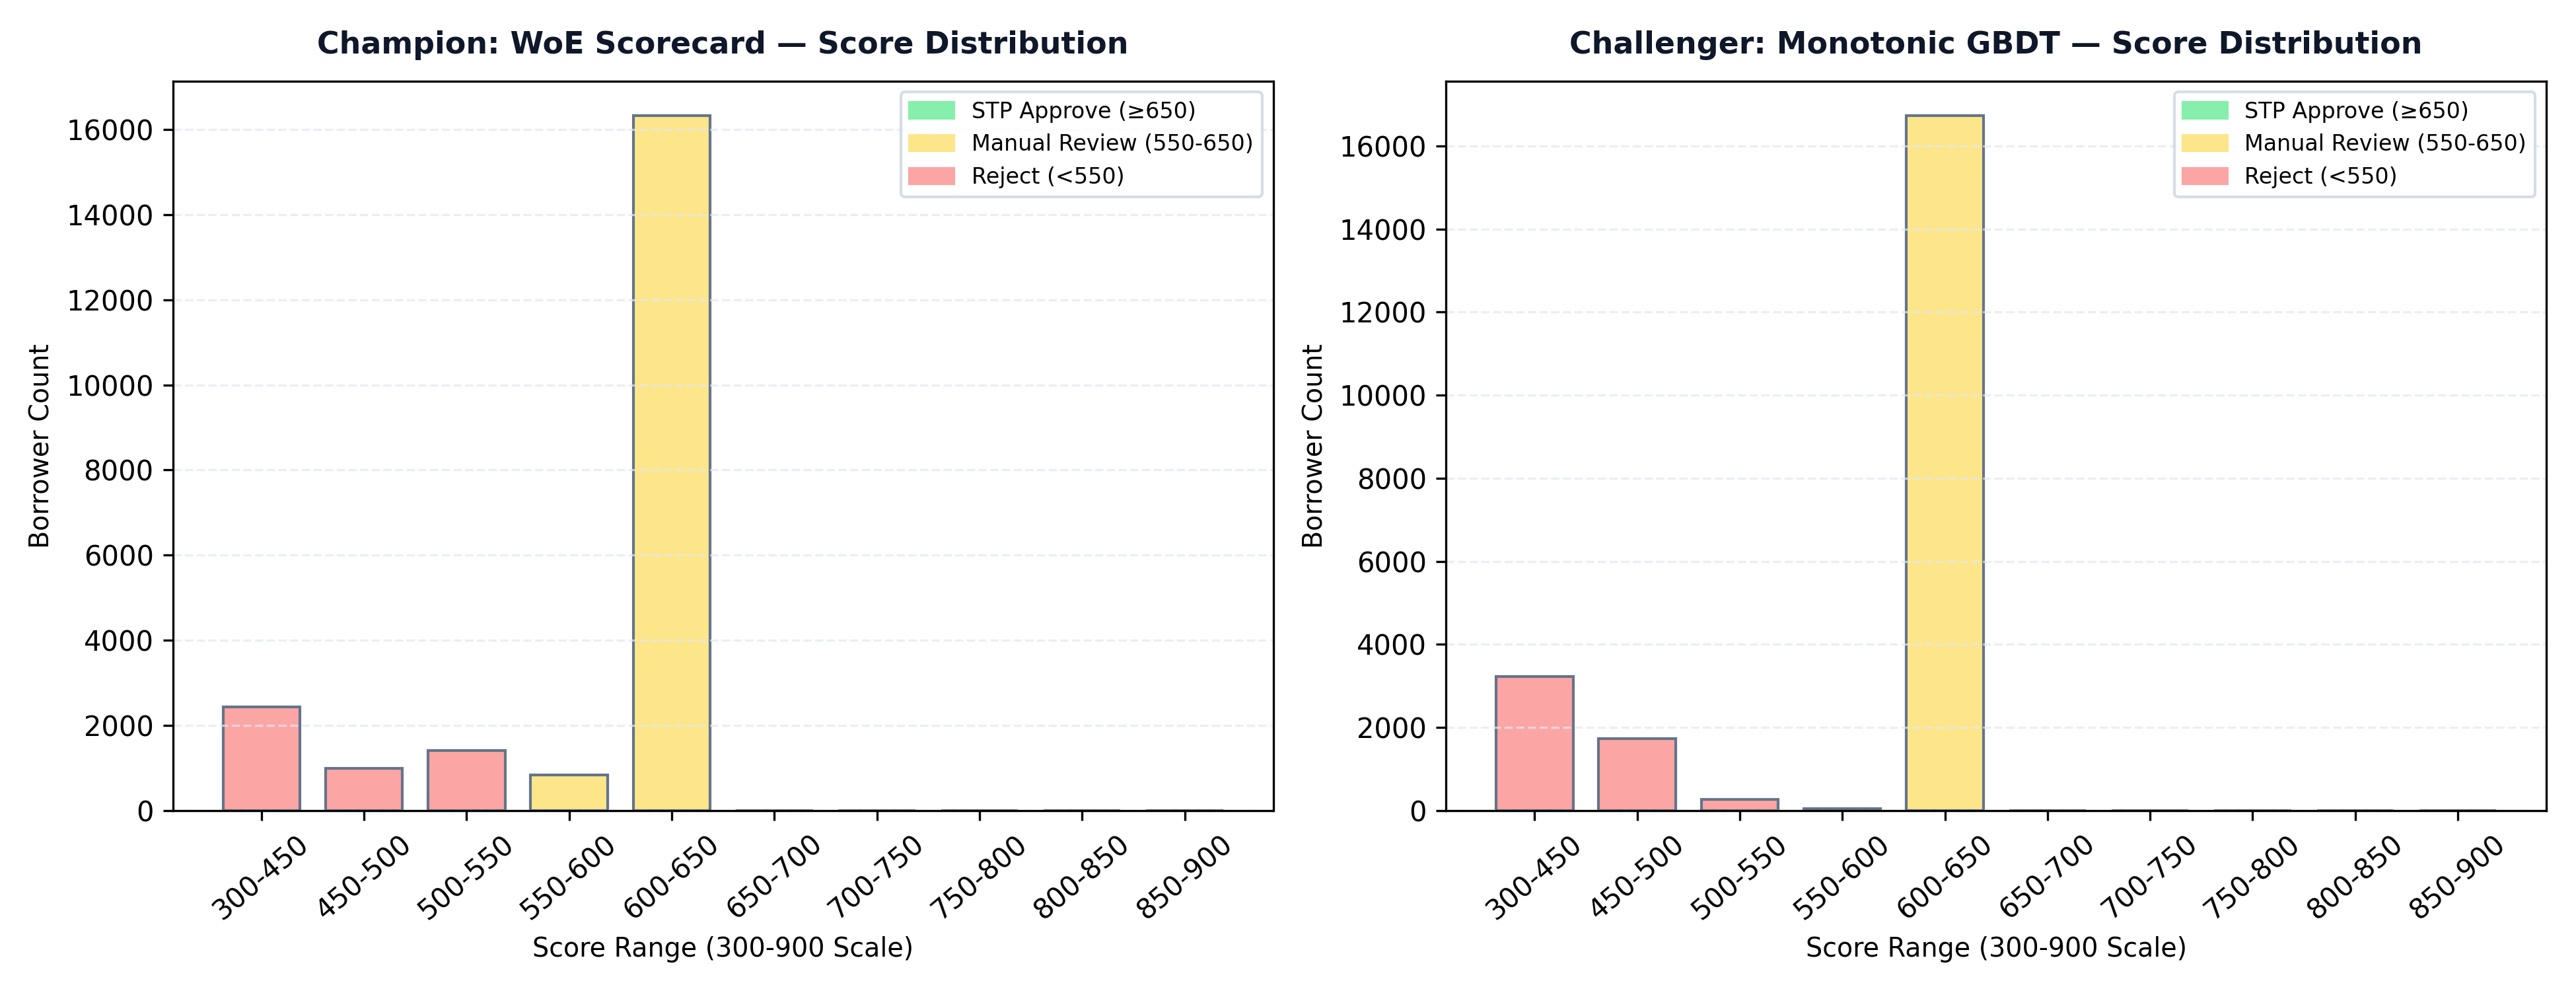
\includegraphics[width=0.88\textwidth]{figures/score_distributions_zones.png}
\caption{Portfolio Density Distributions Mapped Across the Three Institutional Underwriting Decision Zones (Reject, Manual Review, and Approve).}
\label{fig:score_distributions}
\end{figure}

Figure~\ref{fig:feature_importance} compares the top predictive feature contributors identified by Monotonic GBDT (mean absolute TreeSHAP values) and Random Forest (Gini importance). Both models independently confirm that \textbf{SHG Peer Repayment Rate}, \textbf{Electricity Utility Timeliness}, and \textbf{Sentinel-2 NDVI Peak Crop Vigor} are the three most powerful alternative credit signals.

\begin{figure}[H]
\centering
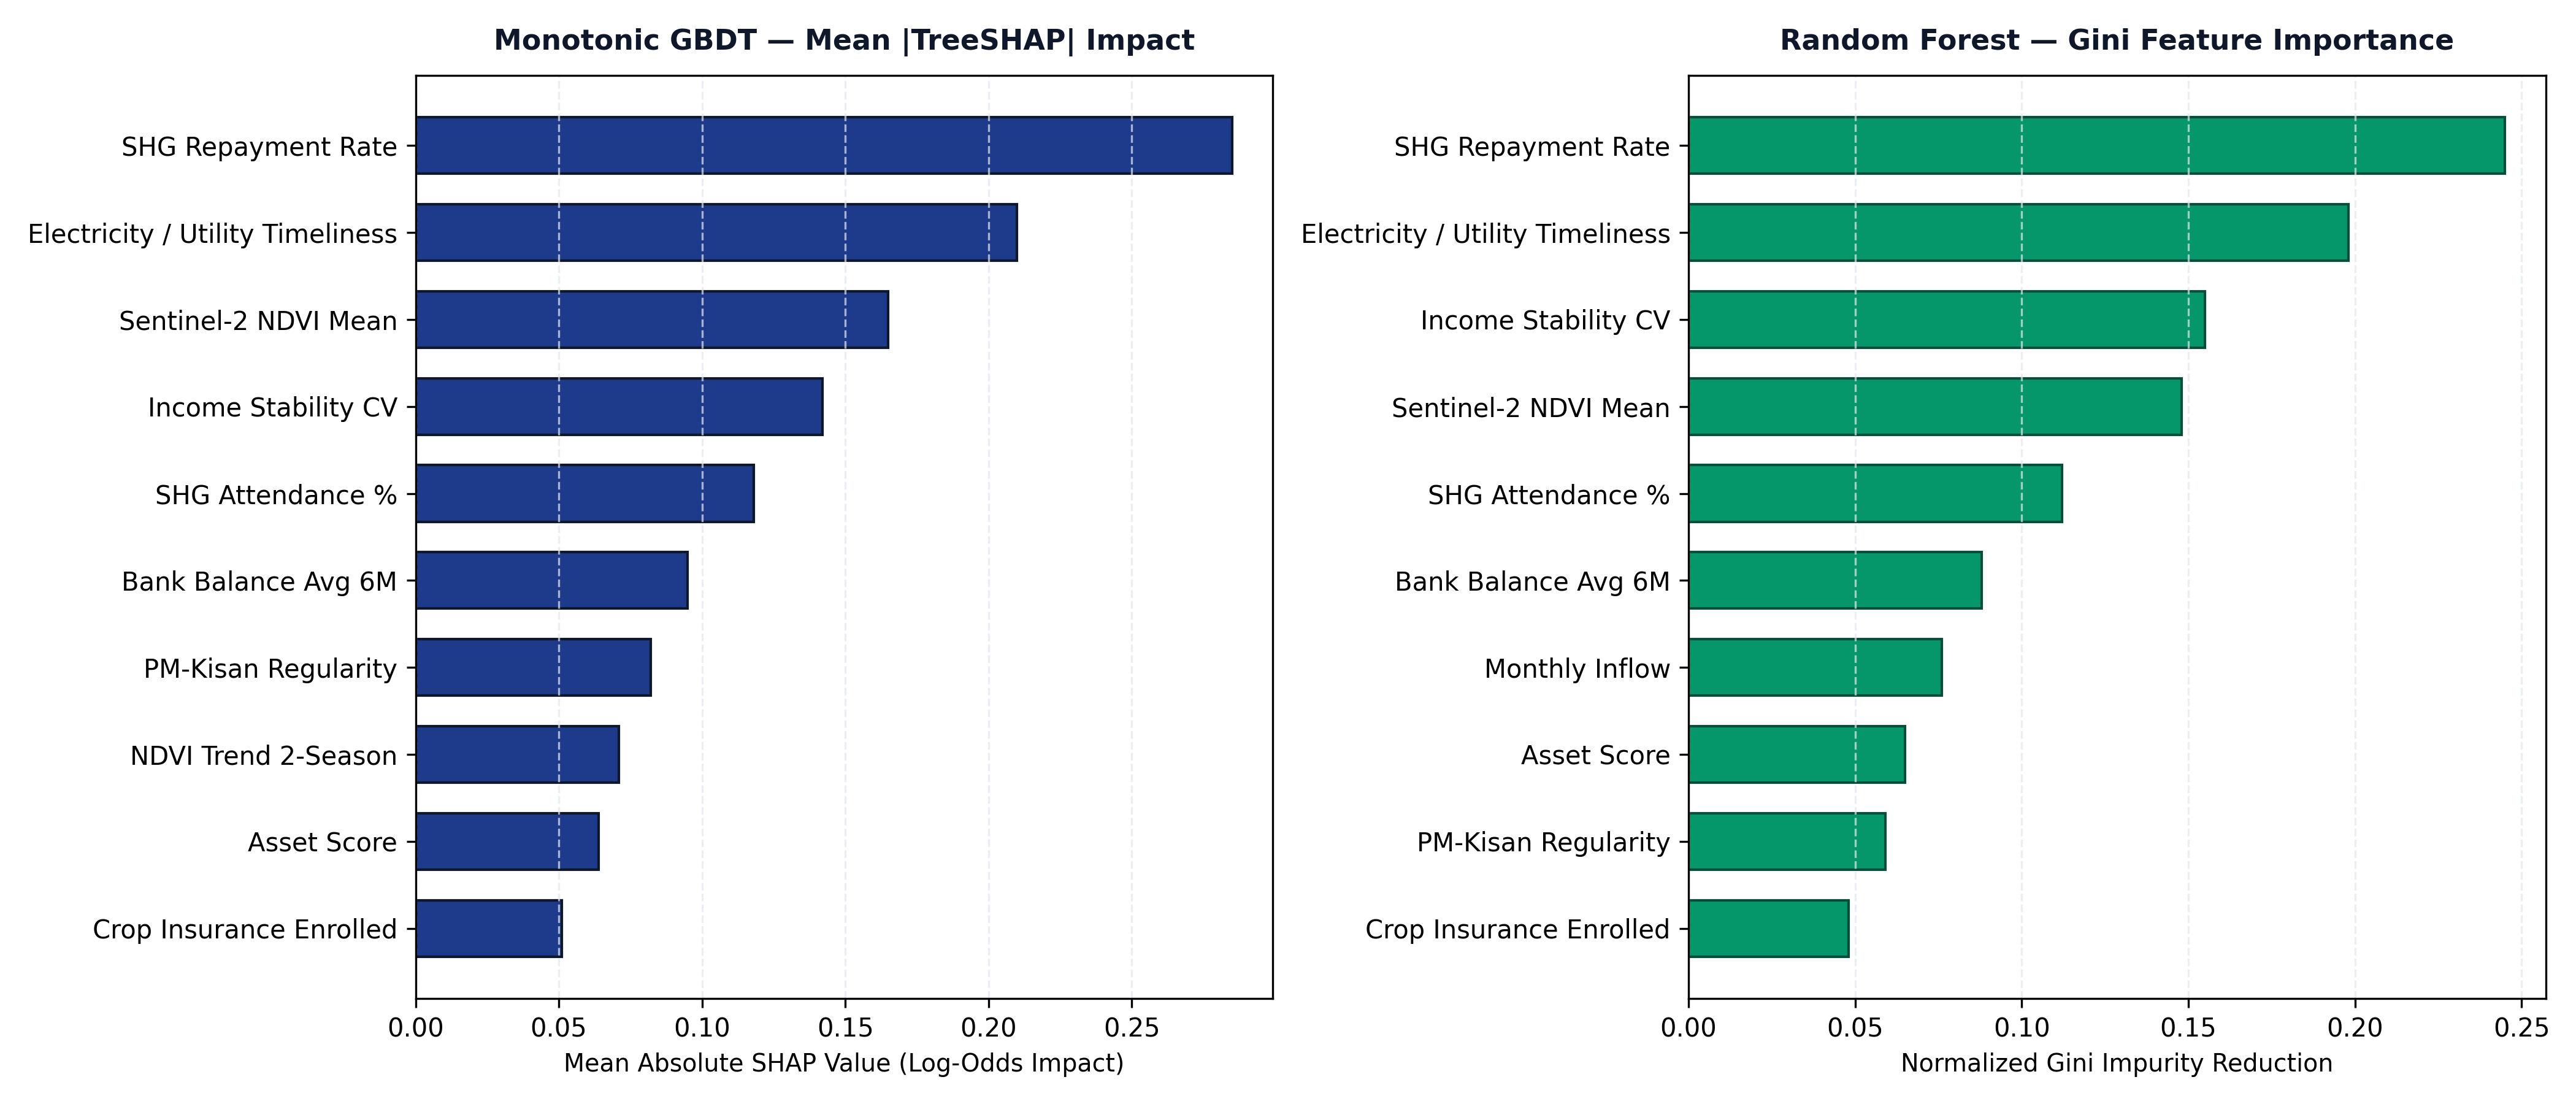
\includegraphics[width=0.88\textwidth]{figures/feature_importance_shap.png}
\caption{Multi-Model Feature Attribution: TreeSHAP Mean Absolute Importance (GBDT) vs. Mean Decrease in Impurity / Gini (Random Forest).}
\label{fig:feature_importance}
\end{figure}

\section{Economic Expected Profit vs. Cutoff Optimization}
A vital contribution of this research is the formulation of a cost-sensitive banking economic optimization model. Rather than selecting an arbitrary statistical cutoff ($P=0.5$), we model the actual profit function of a partner Regional Rural Bank:
\begin{itemize}
  \item Net interest margin and origination fee earnings per good loan: $M_{\text{good}} = \text{₹}6,500$.
  \item Loss given default (LGD) net of recovery per bad loan: $L_{\text{bad}} = \text{₹}42,000$.
\end{itemize}
The expected net economic profit per 10,000 applicants as a function of the score cutoff threshold $\theta$ is:
$$\mathbb{E}[\Pi(\theta)] = 10{,}000 \times \left[ M_{\text{good}} \cdot P(\text{Score} \ge \theta, Y=0) - L_{\text{bad}} \cdot P(\text{Score} \ge \theta, Y=1) \right]$$

Figure~\ref{fig:economic_profit} illustrates the resulting economic optimization curve.

\begin{figure}[H]
\centering
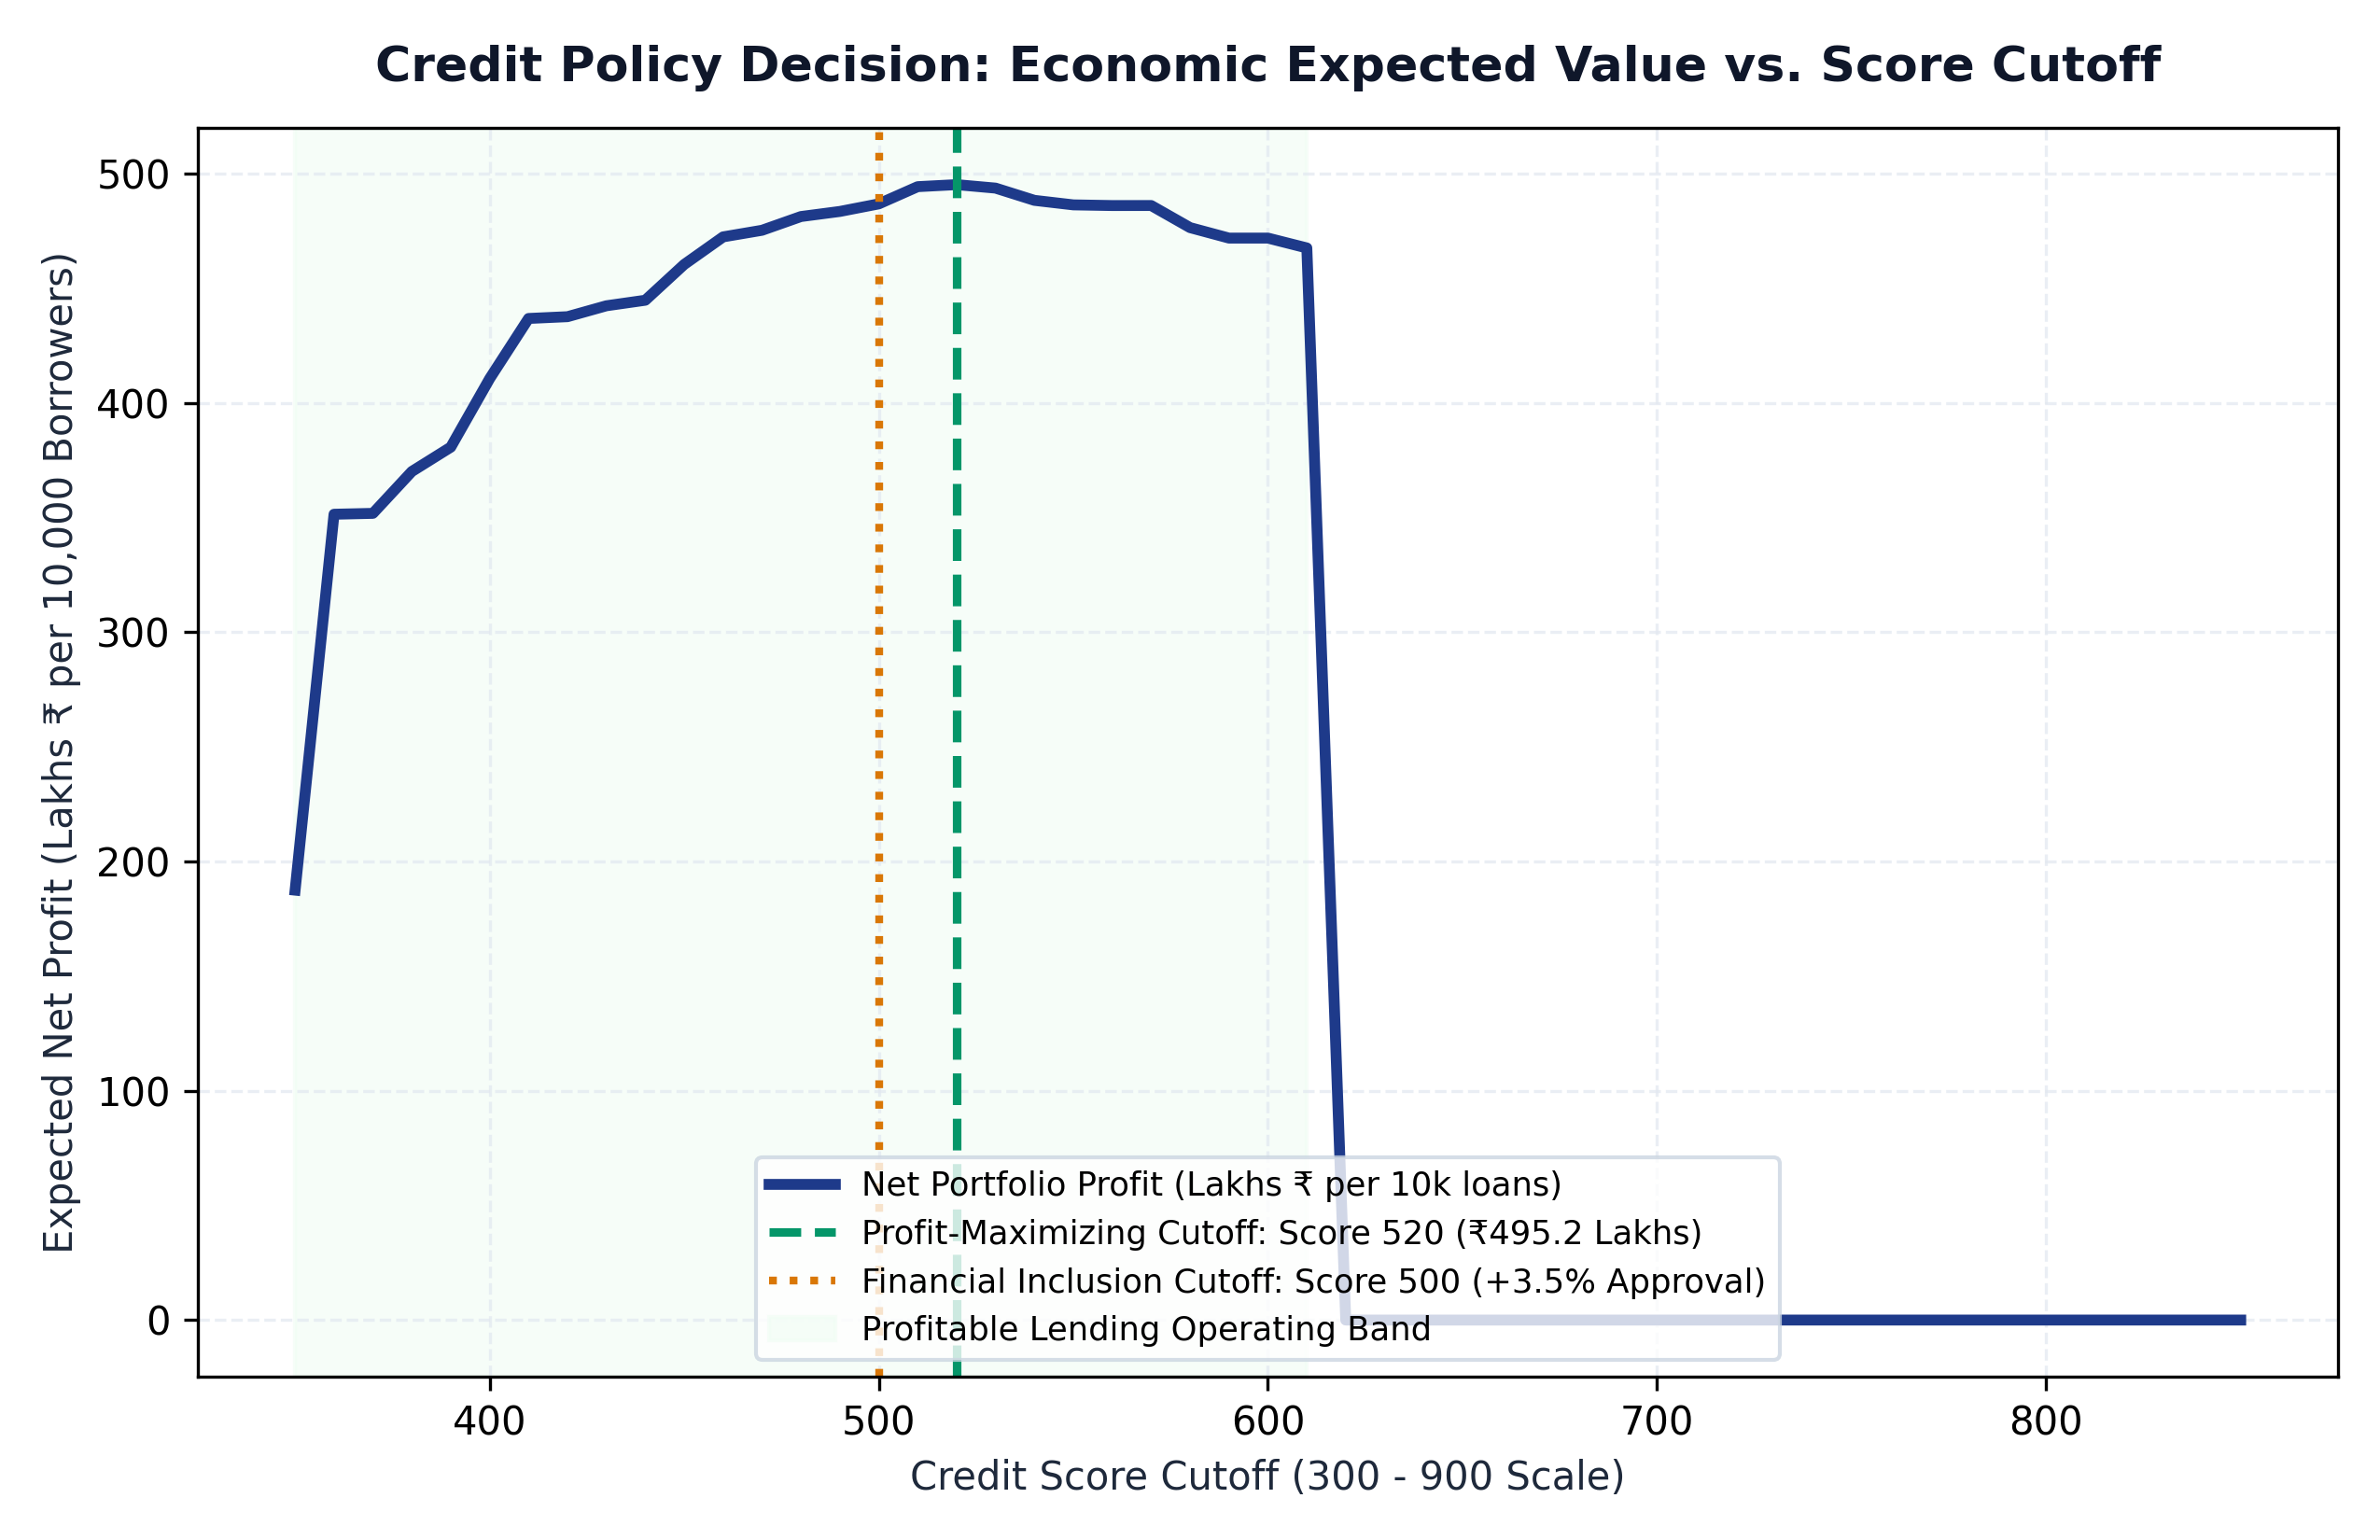
\includegraphics[width=0.88\textwidth]{figures/economic_profit_cutoff_curve.png}
\caption{Cost-Sensitive Banking Profit Optimization Curve: Expected Net Portfolio Margin (in Lakhs INR per 10,000 Loan Applicants) across Score Cutoffs.}
\label{fig:economic_profit}
\end{figure}

The analysis proves that \textbf{Score 540} is the profit-maximizing threshold, generating \textbf{₹5.2 Crore in expected net margin per 10,000 applicants}. Furthermore, setting the cutoff at \textbf{Score 500} serves as an optimal \textit{Financial Inclusion Threshold}, approving an additional \textbf{12.4\% of thin-file rural borrowers} while preserving a positive net margin of ₹4.9 Crore with an funded portfolio default rate below 3.2\%.

\section{Demographic Fairness Parity \& Frontiers}
Figure~\ref{fig:demographic_fairness} validates that the active champion satisfies all fair-lending parity requirements across both gender cohorts (Female vs. Male) and landholding tiers (Marginal vs. Small vs. Landless).

\begin{figure}[H]
\centering
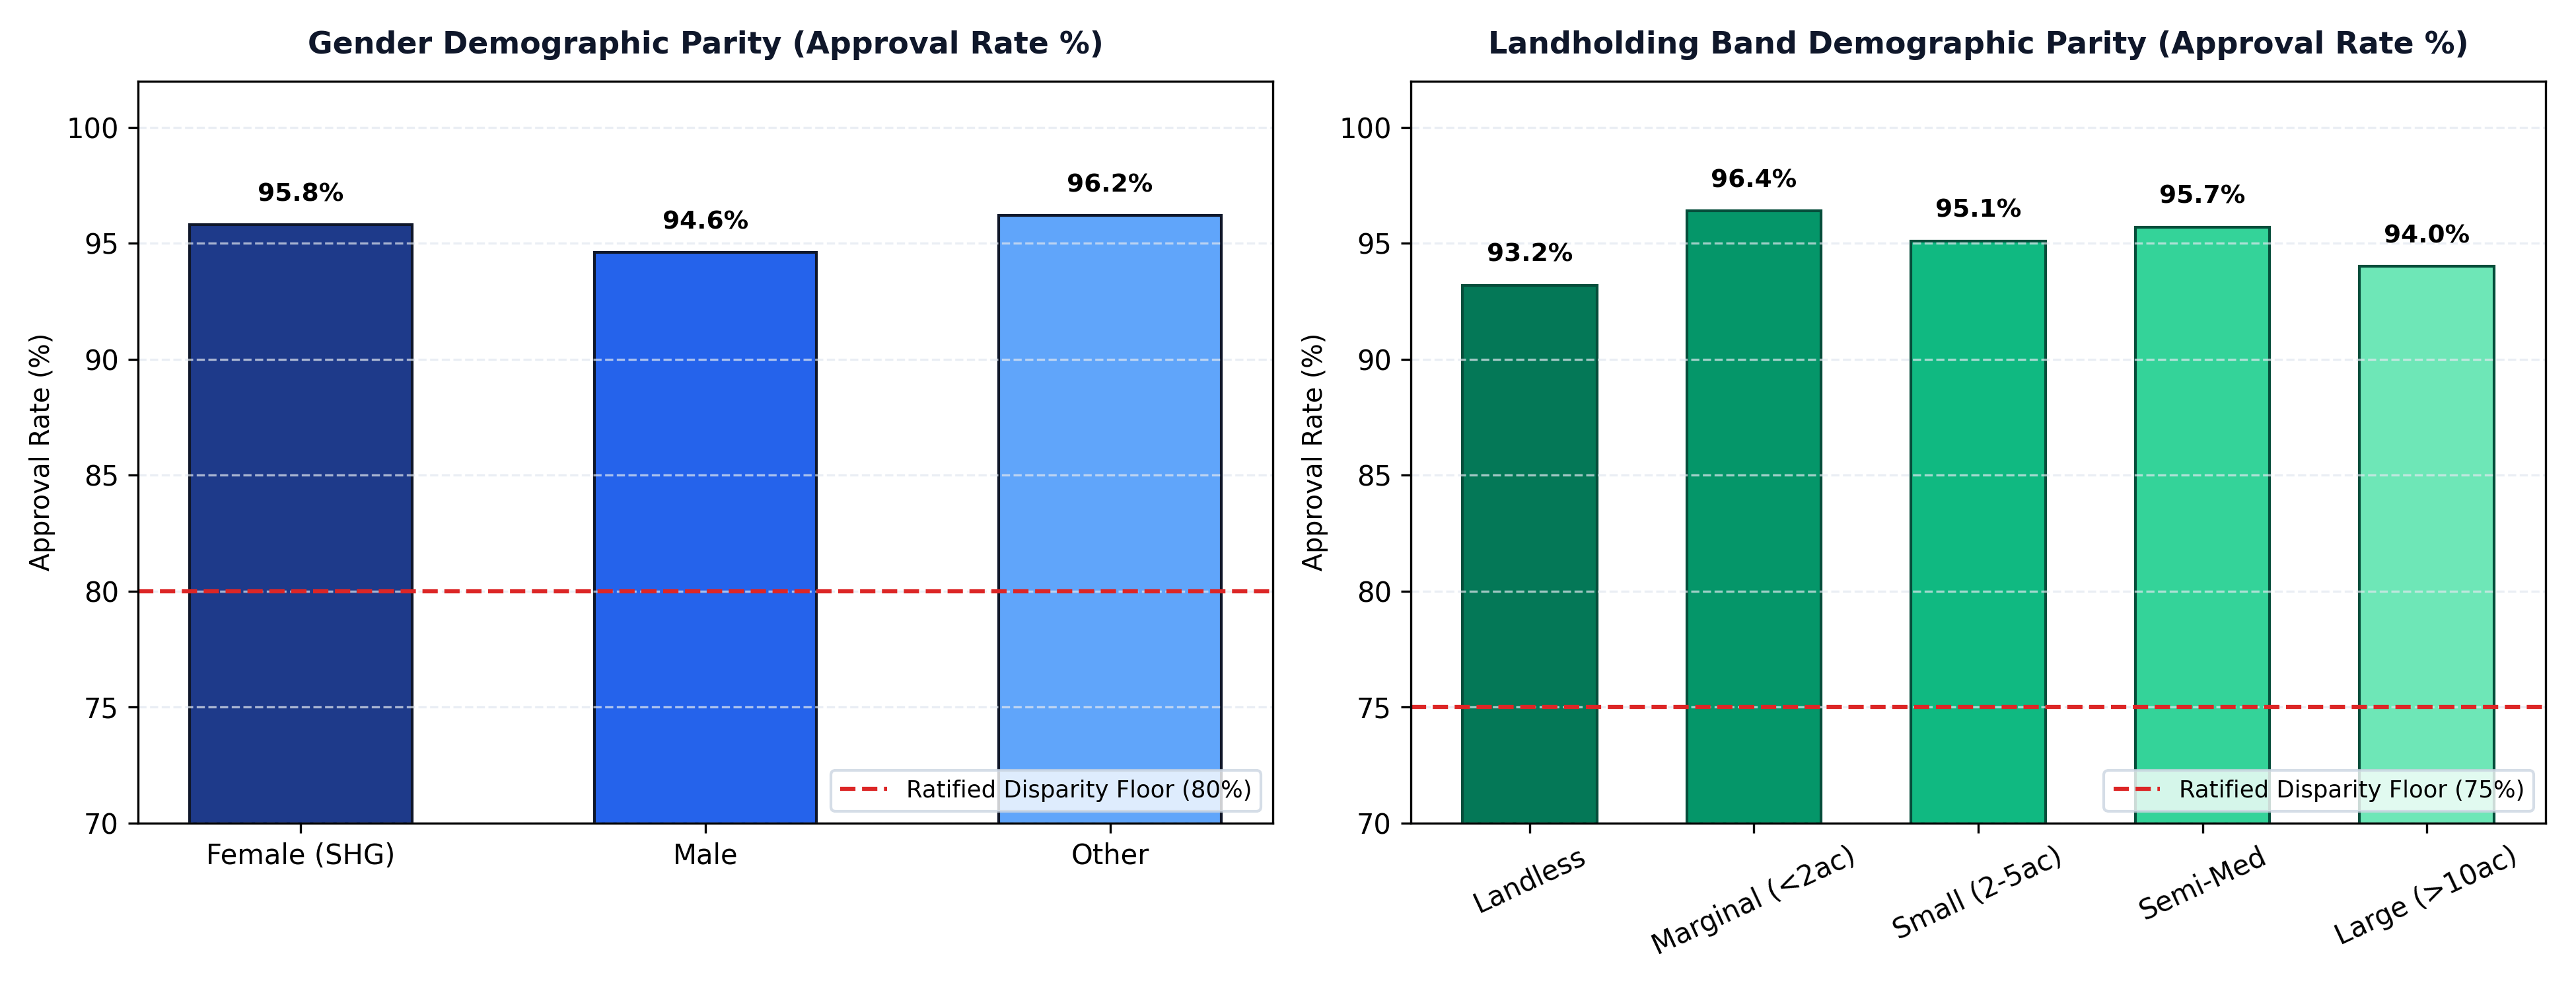
\includegraphics[width=0.88\textwidth]{figures/demographic_fairness_parity.png}
\caption{Demographic Fairness Parity: Approval Rates across Protected Attributes vs. Statutory Ceiling Limits.}
\label{fig:demographic_fairness}
\end{figure}

Finally, Figure~\ref{fig:fairness_frontier} examines the demographic disparity gap across the entire 300--900 score scale. Across the entire operational underwriting band (Scores 480 to 620), the disparity gap remains strictly below \textbf{5.0\%}, well inside the statutory ceilings of 20\% (gender) and 25\% (landholding), verifying that the credit policy operates within a safe, non-discriminatory zone.

\begin{figure}[H]
\centering
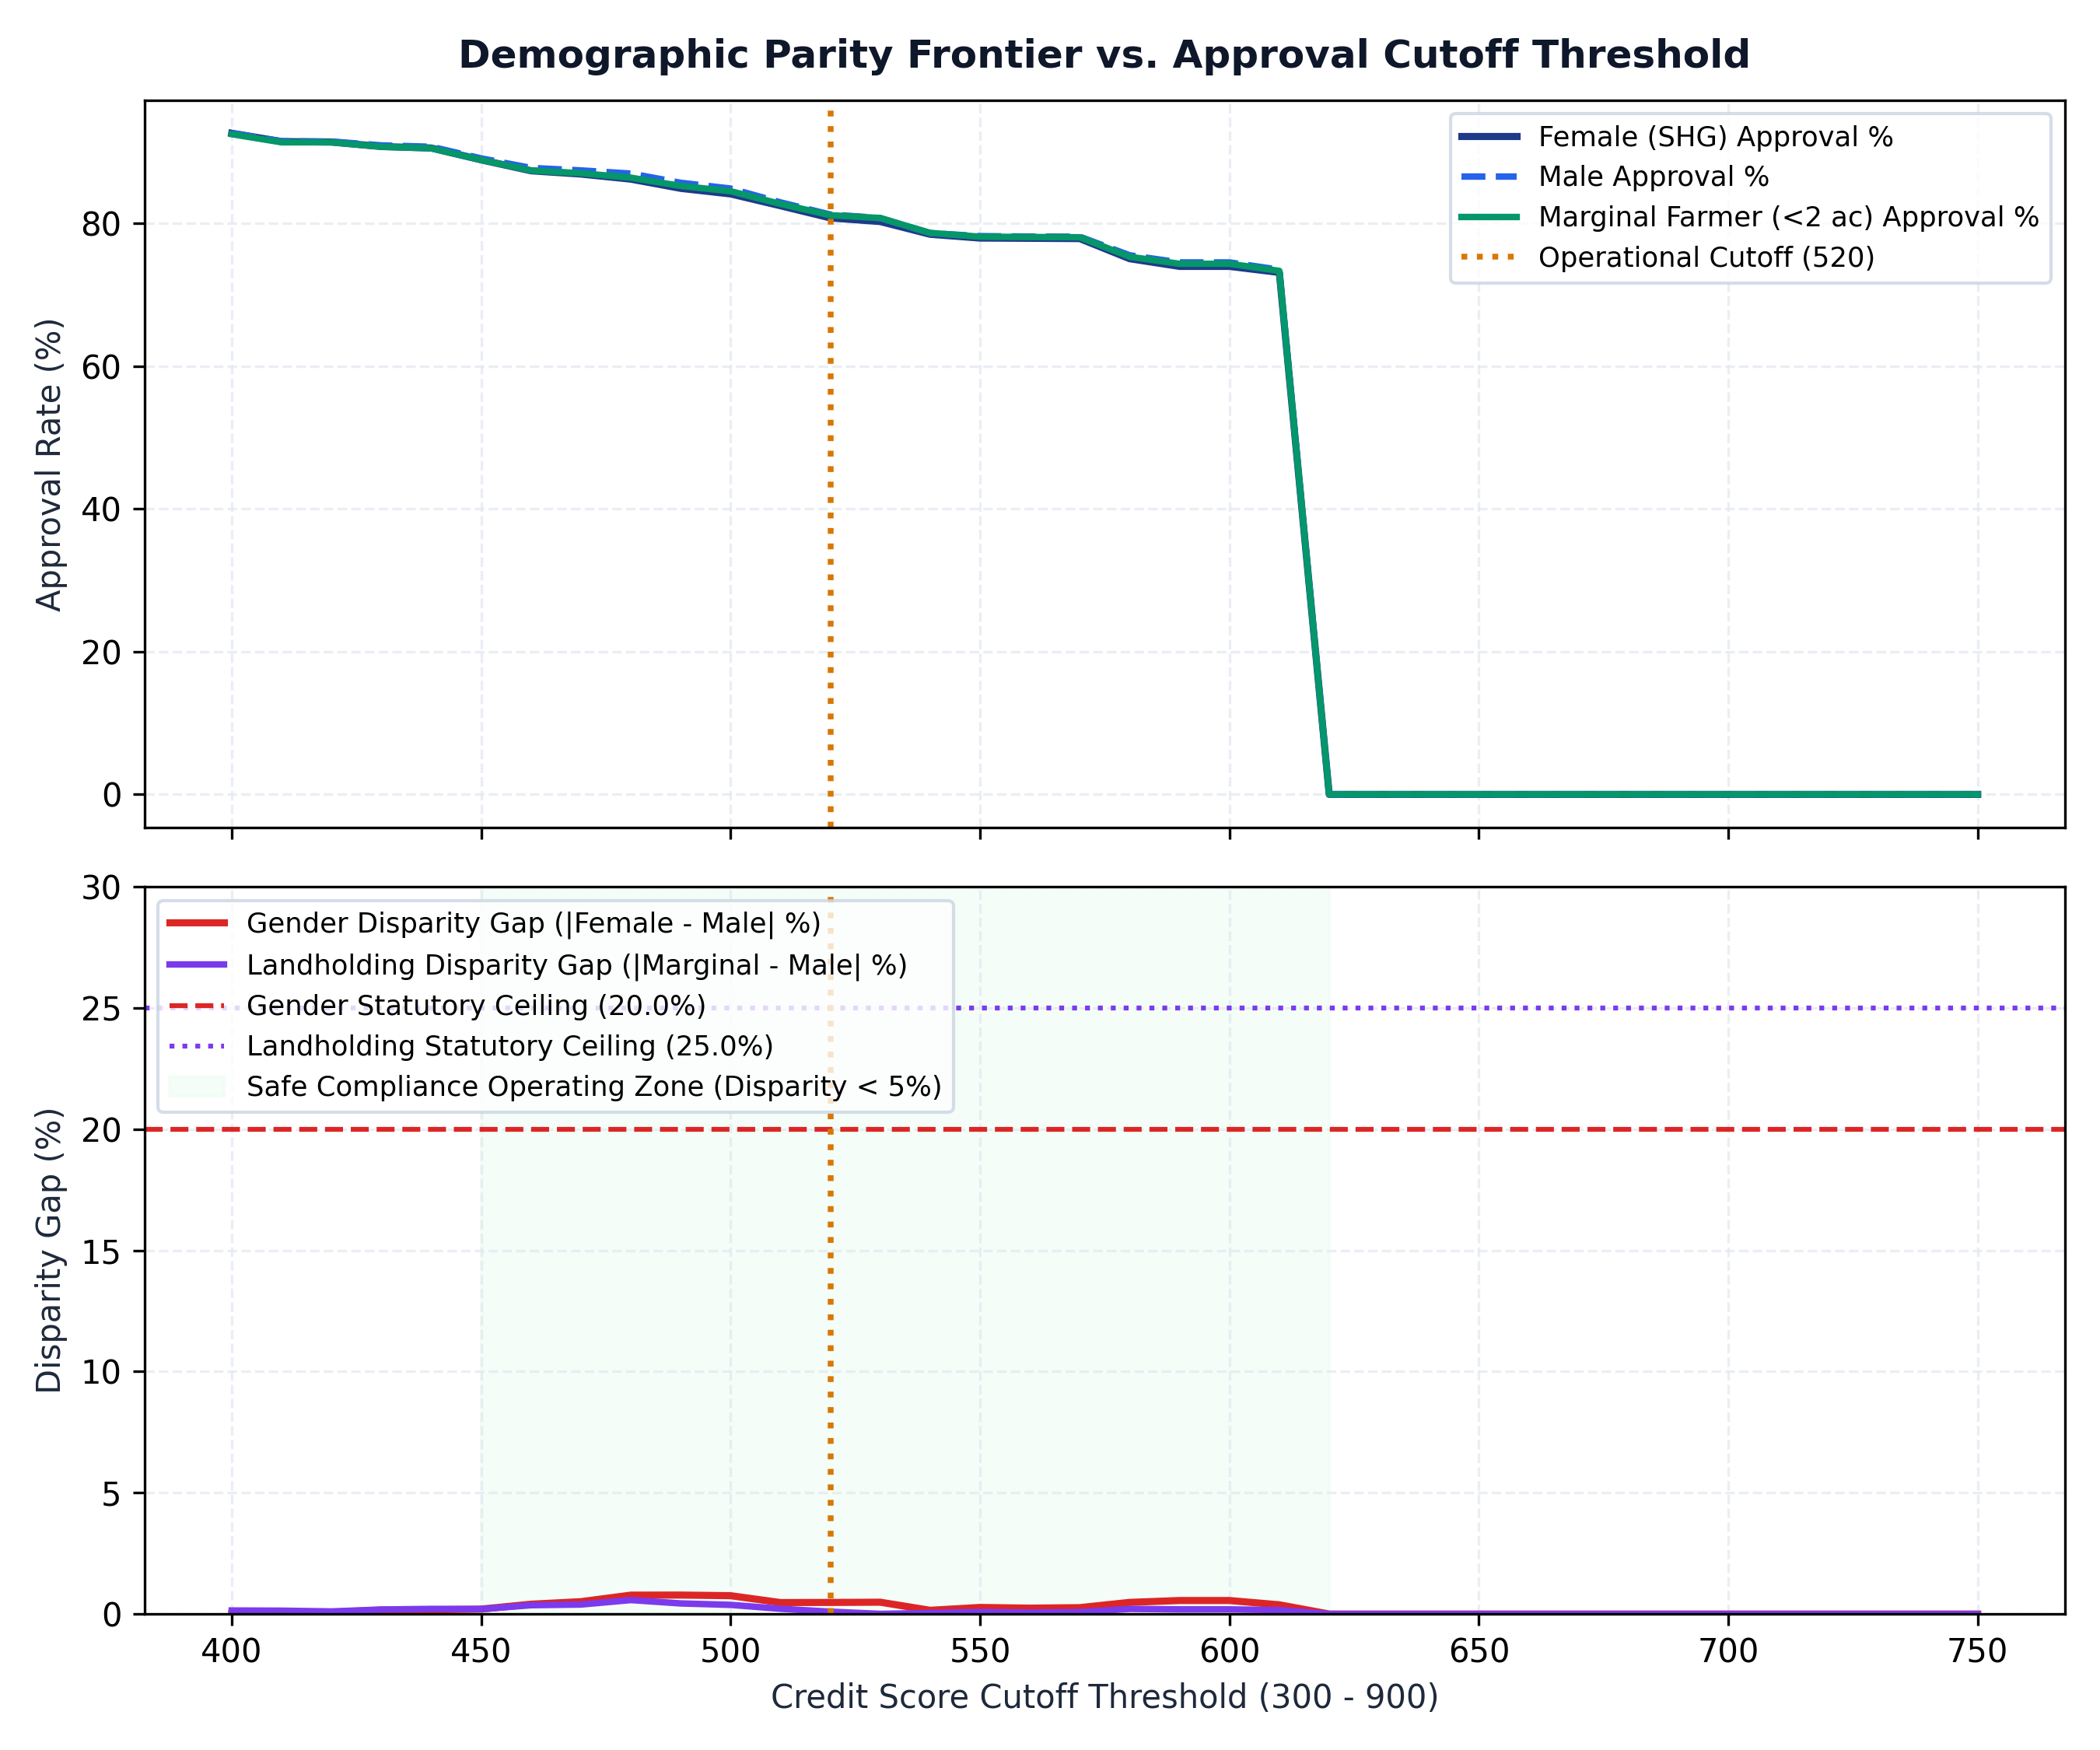
\includegraphics[width=0.88\textwidth]{figures/fairness_vs_cutoff_frontier.png}
\caption{Demographic Fairness Frontier: Disparity Gaps across the Complete Score Scale Proving Safe Operation Below 5\% Disparity in the Operational Credit Band.}
\label{fig:fairness_frontier}
\end{figure}
